% ****** Start of file apssamp.tex ******}
%
%   This file is part of the APS files in the REVTeX 4.1 distribution.
%   Version 4.1r of REVTeX, August 2010
%
%   Copyright (c) 2009, 2010 The American Physical Society.
%
%   See the REVTeX 4 README file for restrictions and more information.
%
% TeX'ing this file requires that you have AMS-LaTeX 2.0 installed
% as well as the rest of the prerequisites for REVTeX 4.1
%
% See the REVTeX 4 README file
% It also requires running BibTeX. The commands are as follows:
%
%  1)  latex apssamp.tex
%  2)  bibtex apssamp
%  3)  latex apssamp.tex
%  4)  latex apssamp.tex
%
\documentclass[reprint,
superscriptaddress,
%groupedaddress,
%unsortedaddress,
%runinaddress,
%frontmatterverbose,
%preprint,
%showpacs,preprintnumbers,
%nofootinbib,
%nobibnotes,
%bibnotes,
amsmath,amssymb,
%  prl,
aps,
%pra,
prb,
%rmp,
%prstab,
%prstper,
%floatfix,
]{revtex4-1}
\usepackage{graphicx}% Include figure files
\usepackage[caption=false]{subfig}
\captionsetup[subfigure]{labelformat=brace}
%\usepackage{dcolumn}% Align table columns on decimal point
\usepackage{bm}% bold math
\usepackage{hyperref}
\usepackage{xargs}% Use more than one optional parameter in a new commands
\usepackage{xcolor,ulem}% Coloured text etc.
\usepackage[colorinlistoftodos,prependcaption,textsize=tiny]{todonotes}
\newcommandx{\unsure}[2][1=]{\todo[linecolor=red,backgroundcolor=red!25,bordercolor=red,#1]{#2}}
\newcommandx{\change}[2][1=]{\todo[linecolor=blue,backgroundcolor=blue!25,bordercolor=blue,#1]{#2}}
\newcommandx{\info}[2][1=]{\todo[linecolor=OliveGreen,backgroundcolor=OliveGreen!25,bordercolor=OliveGreen,#1]{#2}}
\newcommandx{\improve}[2][1=]{\todo[linecolor=green,backgroundcolor=green!25,bordercolor=green,#1]{#2}}
\newcommandx{\thiswillnotshow}[2][1=]{\todo[disable,#1]{#2}}

\newcommand{\ket}[1]{$\left|#1\right\rangle$}
\newcommand{\Ket}[1]{\left|#1\right\rangle}
%voor gebruik in text
\newcommand{\bra}[1]{$\langle #1\rvert$}
%voor gebruik binnen equation environment
\newcommand{\Bra}[1]{\langle #1\rvert}
\newcommand{\kpoint}{$\bold{K}$ }
\newcommand{\Kpoint}{$\bold{K'}$ }
\newcommand{\gpoint}{$\bold{\Gamma}$}
\newcommand{\angstrom}{\mbox{\normalfont\AA} }
\newcommand{\sa}[1]{{\color{violet}[#1]}}
\newcommand{\lp}[1]{{\color{red}[#1]}}
\begin{document}
\title{First-principles theory of giant Rashba-like spin splitting in bulk Germanium Telluride}
\author{Louis Ponet}
\email{louis.ponet@iit.it}
\affiliation{%
 Quantum Materials Theory, Istituto Italiano di Tecnologia, Genoa 16163, Italy
}
\affiliation{Department of Nanosciences, Scuola Normale Superiore di Pisa 56100, Italy}
\author{S. Artyukhin}%
 \email{sergey.artyukhin@iit.it}
\affiliation{%
 Quantum Materials Theory, Istituto Italiano di Tecnologia, Genoa 16163, Italy
}
\date{\today}
\begin{abstract}
Large Rashba-like spin splitting has been recently found in the band structure of certain bulk ferroelectrics. In contrast to the relativistic Rashba effect, the chiral spin texture and large spin splitting of the electronic bands depend strongly on the character of the band and atomic spin-orbit coupling.
We establish that this can be traced back to an interplay between the orbital angular momentum and ferroelectricity. The additional dependence on the orbital composition of the bands is crucial to the complete picture of the effect. Results from first-principles calculations on ferroelectic GeTe verify the key predictions of the model.
\end{abstract}

\pacs{Valid PACS appear here}% PACS, the Physics and Astronomy
% Classification Scheme.
\maketitle
\section{Introduction}
% Bulk ferroelectrics with large atomic spin-orbit coupling allow for electric control of spin-polarized states~\cite{DiSante2013,Ishizaka2011,Kim2014, Liebmann2016, Krempasky2015SurfaceSemiconductor}, allowing for the switching of the spin texture by an externally applied electric field. 
% The underlying mechanism is, however, not well understood.
The research area of spintronics aims to supersede electronics  by using spins instead of charges for information processing and storage. %\sa{https://doi.org/10.1146/annurev-conmatphys-070909-104123} 
Many possible devices that utilize both charge and spin degrees of freedom of carriers have been theorized. Examples are the spin field-effect transistors (spin-FET)\cite{Datta1990}, storage devices which utilize spin-current and associated spin-transfer torque to efficiently manipulate magnetic domains \cite{Kent2015,Jungwirth2016}. In spite of fundamental interest and potential for applications, the actual realization of these devices has been rather elusive. One of the main culprits for the limited success to date is that the devices require very granular, ideally electric, control of the spin, which is impeded by widely separated energy scales and weak coupling between magnetic and structural degrees of freedom. One class of materials that allow for such electric control of spin-polarized states are the ferroelectric semiconductors with large atomic spin-orbit coupling (SOC) \cite{DiSante2013,Ishizaka2011,Kim2014}. The underlying mechanism is a coupling between the spin-polarized states and the ferroelectric polarization of the material that makes it possible to switch the ferroelectric polarization and in turn the polarization of the spin by the external electric field. The effect has been confirmed both experimentally \cite{Ishizaka2011,Liebmann2016,Krempasky2015SurfaceSemiconductor}, and through ab initio density functional theory (DFT) simulations \cite{DiSante2013}. 

This work aims to clarify the effect in bulk systems, the interplay between ferroelectricity, orbital character and atomic SOC that causes it, and in doing so identifies the criteria for finding other materials with large Rashba splitting.
We start with a brief overview of the important properties of GeTe, followed by a qualitative description of the coupling between the orbital angular momentum (OAM) and the electric polarization. Then we verify the model by performing ab initio calculations on germanium telluride (GeTe), a typical example of the aforementioned effects.
\begin{figure}[b]
% ~\centering
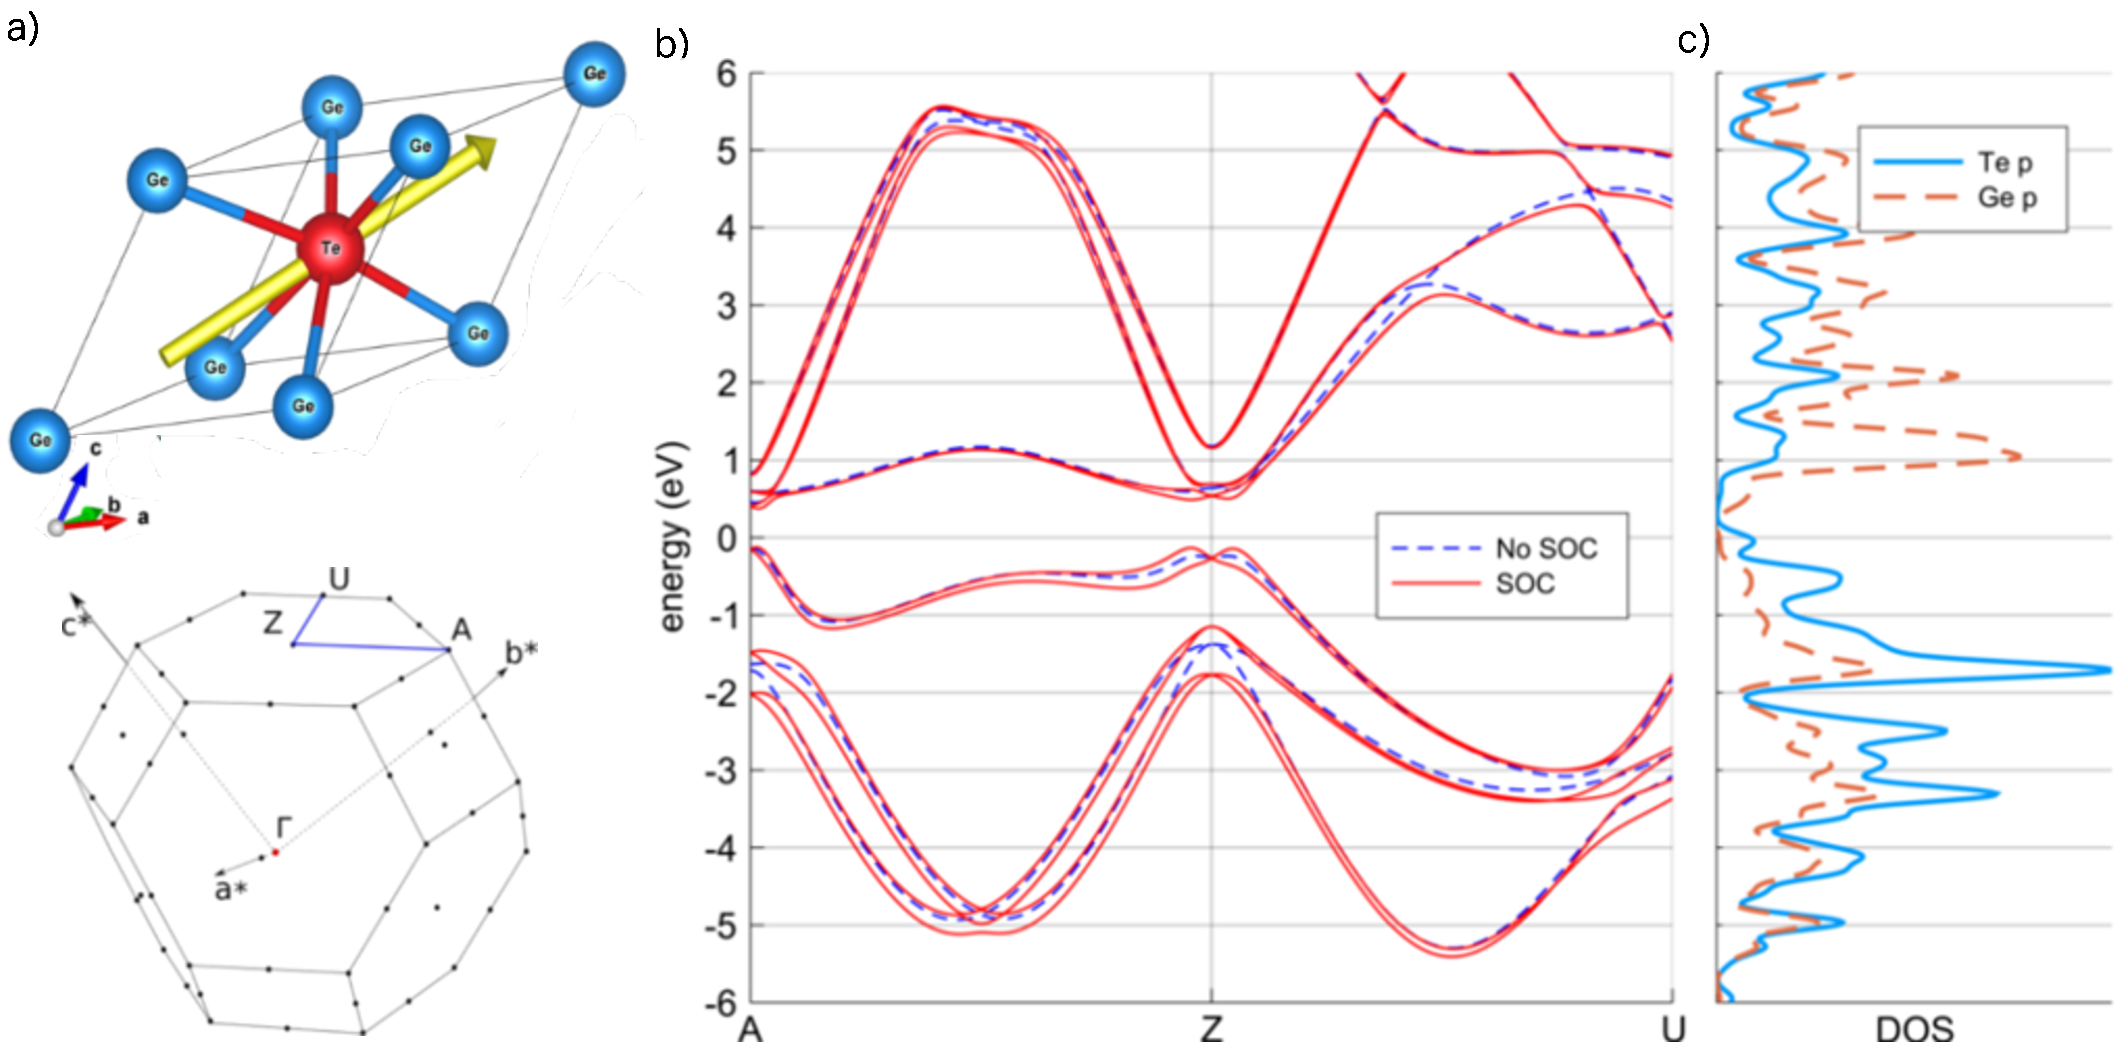
\includegraphics[width=\linewidth]{BZBSDOS.pdf}
\caption{\label{fig:eigvalsdos}(a) Rhombohedral unit cell and Brillouin zone of GeTe, with the polarization direction in yellow. (b) Band structure obtained from a DFT calculation with and without SOC, along the blue path in panel (a). (c) partial DOS for Te and Ge p orbitals computed without SOC.}
\end{figure}
\section{Overview: Germanium Telluride}
Germanium telluride (GeTe) is a ferroelectric semiconductor with R$3m$ space group (\#160 in International Tables). The ferroelectricity is owed to a small displacement along the threefold rotation axis ($z$) of the Te layers towards one of the two neighboring Ge layers \cite{Rabe1987}. The resulting electric polarization is therefore also oriented along the $z$ axis, as can be seen in Fig. \ref{fig:eigvalsdos}-(a). The band structure, displayed in Fig. \ref{fig:eigvalsdos}-(b), presents a distinct large linear spin splitting around the $Z$ point, resembling the well known Rashba effect \cite{DiSante2013}. The characteristic splitting is observed both along the $Z-A$ and $Z-U$ directions, but not along $Z-\Gamma$ path, due to time-reversal symmetry of the latter.

The density of states (DOS) is displayed in Fig.~\ref{fig:eigvalsdos}-(c). The valence bands are comprised mostly of Te 5p orbitals, whereas the conduction bands are mostly formed by Ge 4p orbitals. This orbital character of valence and conduction bands, together with the stronger atomic SOC on Te atom, results in a more pronounced spin splitting in the valence bands. We will focus on the first three valence bands, the top one of which mainly has $p_z$ character whereas the two lower bands, which are degenerate at the $Z$-point, are formed by $p_x$ and $p_y$ orbitals. The crystal field splitting between bands of $p_z$ and $p_{x,y}$ characters results from the distortion of the ideal Te-Ge$_6$ octahedron.
\section{Interplay of ferroelectricity, orbital angular momentum and spin-orbit coupling}
% % ~\centering
\begin{figure}[b!]
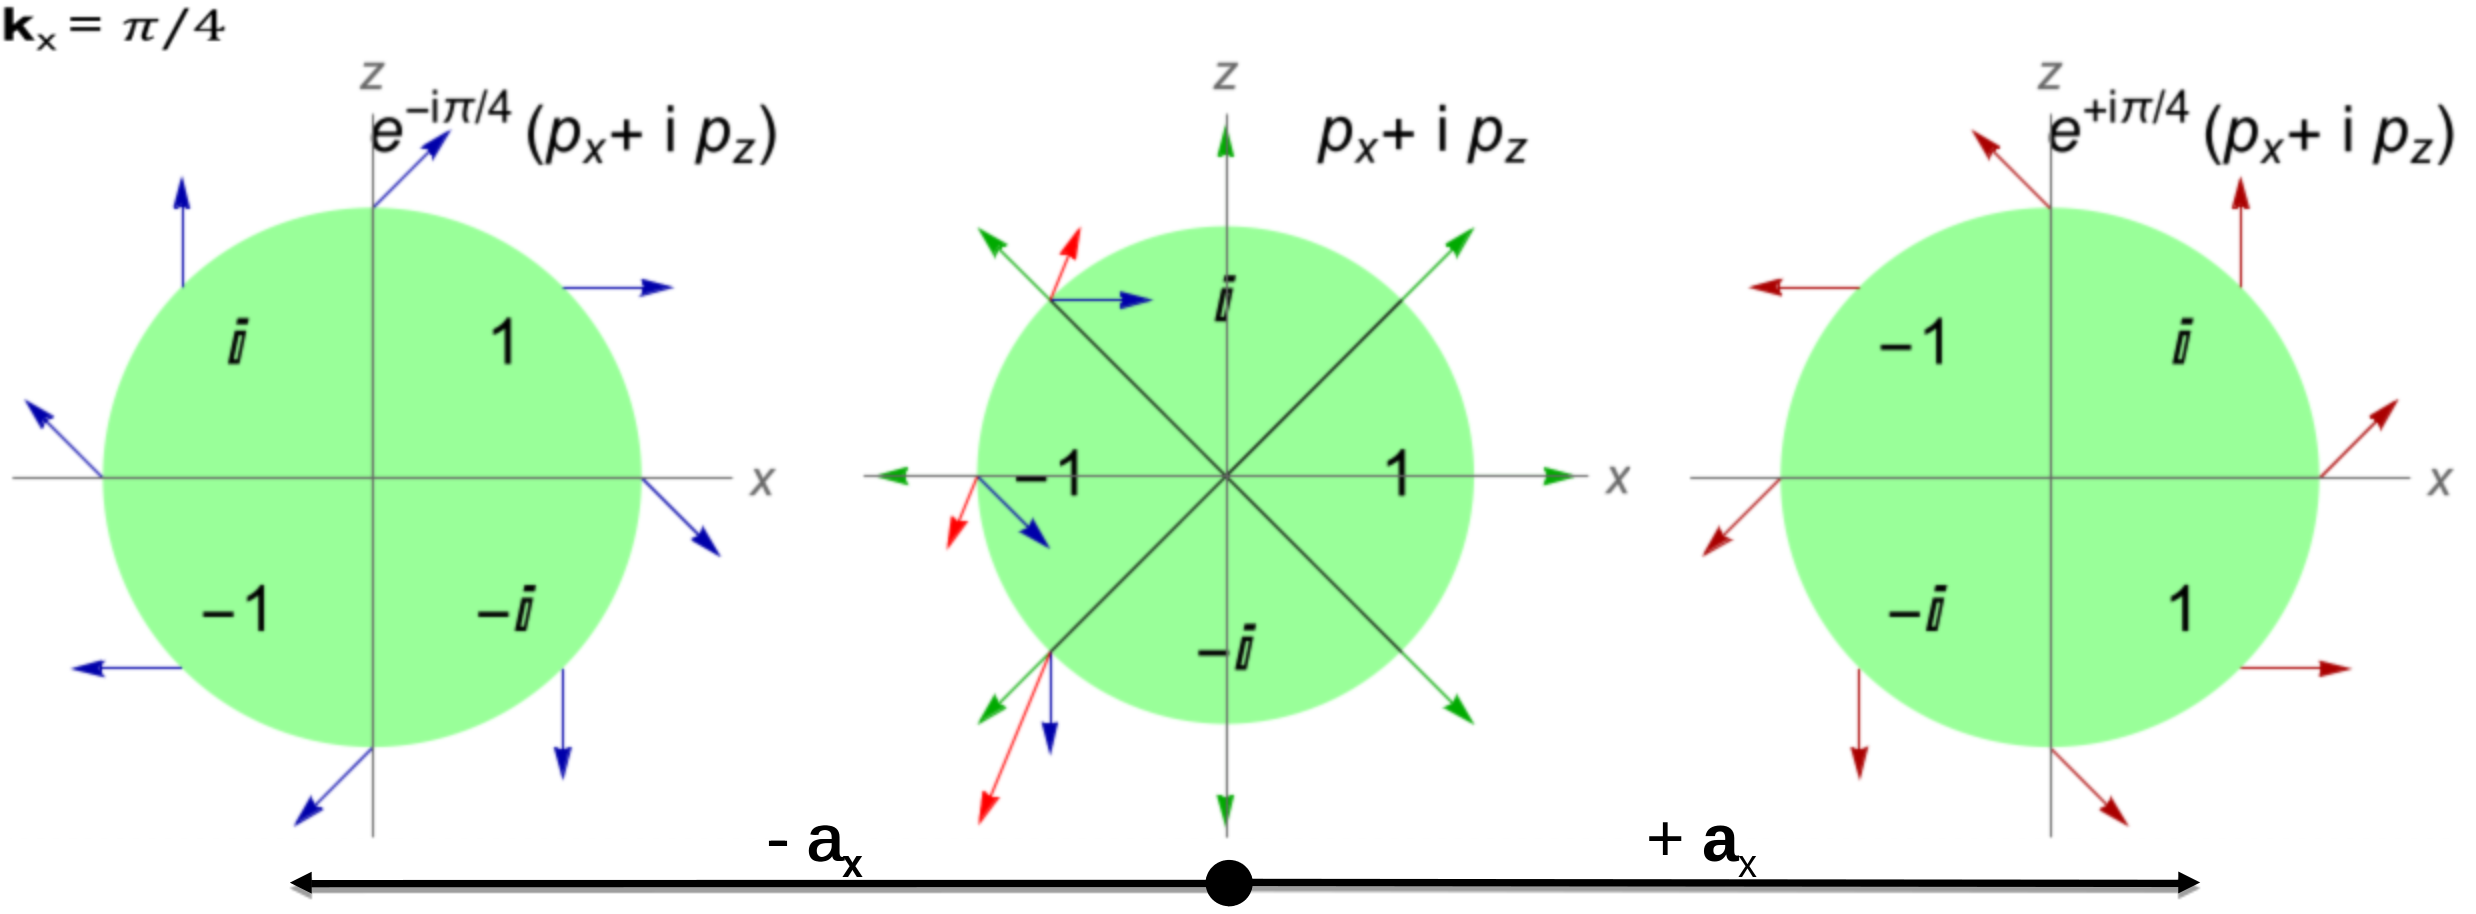
\includegraphics[width=\linewidth]{interference.png}
\caption{\label{fig:interference}Interference between orbitals with nonzero OAM. Three neighboring unit cells are displayed, each with the same $p_x + ip_z$ orbital (thus having nonzero $l_y$). The wave functions of the left and right unit cells have their phase rotated by the plane-wave part $e^{i k_x R_x}$. The amplitude and phase of the wave function are encoded with the length and polar angle of the arrows.}
\end{figure}
The $k$-dependent spin splitting, shown in Fig.~\ref{fig:eigvalsdos}, could be (incorrectly) attributed to a Rashba effect, described by the relativistic Rashba Hamiltonian \cite{Rashba1959SymmetryAr, Lifshitz1982CourseTheory},
\begin{equation}\label{eq:relrashba}
\mathcal{H}_R=\alpha_R (\bm{k} \times \bm{E})\cdot \bm{\sigma}, \quad \alpha_R=\frac{e\hbar^2}{2m^2c^2},
\end{equation}
where $\bm{E}$ originates from the ferroelectric polarization in the open circuit configuration, and with an abnormally large $\alpha_R\approx 30.7$~eV\.\angstrom \cite{DiSante2013}, while in the vacuum  $\alpha_R=10^{-6}$~eV. However, all known proper ferroelectrics do not support the polarization in an open boundary situation, where depolarizing fields are not screened \cite{Garrity2013Hyperferroelectrics:Polarization}.
Secondly, it is a well known fact that the periodic boundary conditions for the potential used in DFT imply short circuit electric boundary conditions\cite{Meyer2008AbFields}, $\bm E=0$, causing the relativistic effect (\ref{eq:relrashba})to vanish.

Another issue, as has been experimentally confirmed\cite{Krempasky2015SurfaceSemiconductor}, is that the orientation of the spin polarization of the spin-split subbands depends on the atomic orbitals that form the band.
This is not accounted for by the relativistic Rashba effect, where the orientation of spin-polarization is uniquely defined by the vector product of the wave vector and the inversion symmetry breaking field (in our case the electric polarization).
The last discrepancy is that the splitting depends strongly on the atomic SOC.
It is then evident that the mechanism behind the spin splitting must be one that couples the atomic character of the bands (and their respective atomic SOC) to the electric polarization.
In their seminal papers Park {\it et al.}~addressed these issues, focusing on surfaces. The pivotal role of OAM \cite{Park2011,Park2012,Park2015MicroscopicMomentum,Hong2015QuantitativeSplitting} was emphasized and shown to lead to a better description of the spin splitting.
The underlying mechanism is that interference between neighboring atomic orbitals with nonzero OAM in the Bloch function can result in $k$-dependent charge asymmetry as shown in Fig.~\ref{fig:interference}. In the region of overlap between the central and left-shifted wavefunctions, a sum of their phases is shown by the resulting red arrow. This showcases the charge asymmetry due to the interference, creating a dipole along the $z$ axis in this specific case.
The resulting electric dipole then couples to the inversion symmetry-breaking field at the surface, resulting in the splitting of OAM states, linear in $k$.
This effect can also exist in bulk materials, where the inversion symmetry can be broken by, e.g., ferroelectric polarization or an external electric field.


\begin{figure}[t]
~\centering
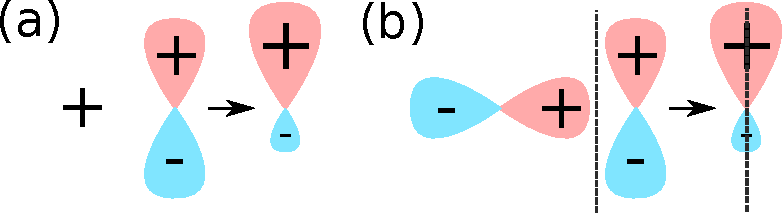
\includegraphics[width=\linewidth]{overlapdip.pdf}\caption{\label{fig:overlapdip} Overlap dipoles of orbitals in neighboring unit cells. (a) Nonzero dipole coming from shifted $p$ orbitals. (b) Dipoles of shifted $d$ orbitals compensate at a high symmetry point.}
\end{figure}
% \begin{figure*}[ht!]
% \centering
% \begin{subfigure}[b]{0.49\textwidth}
% \centering
% 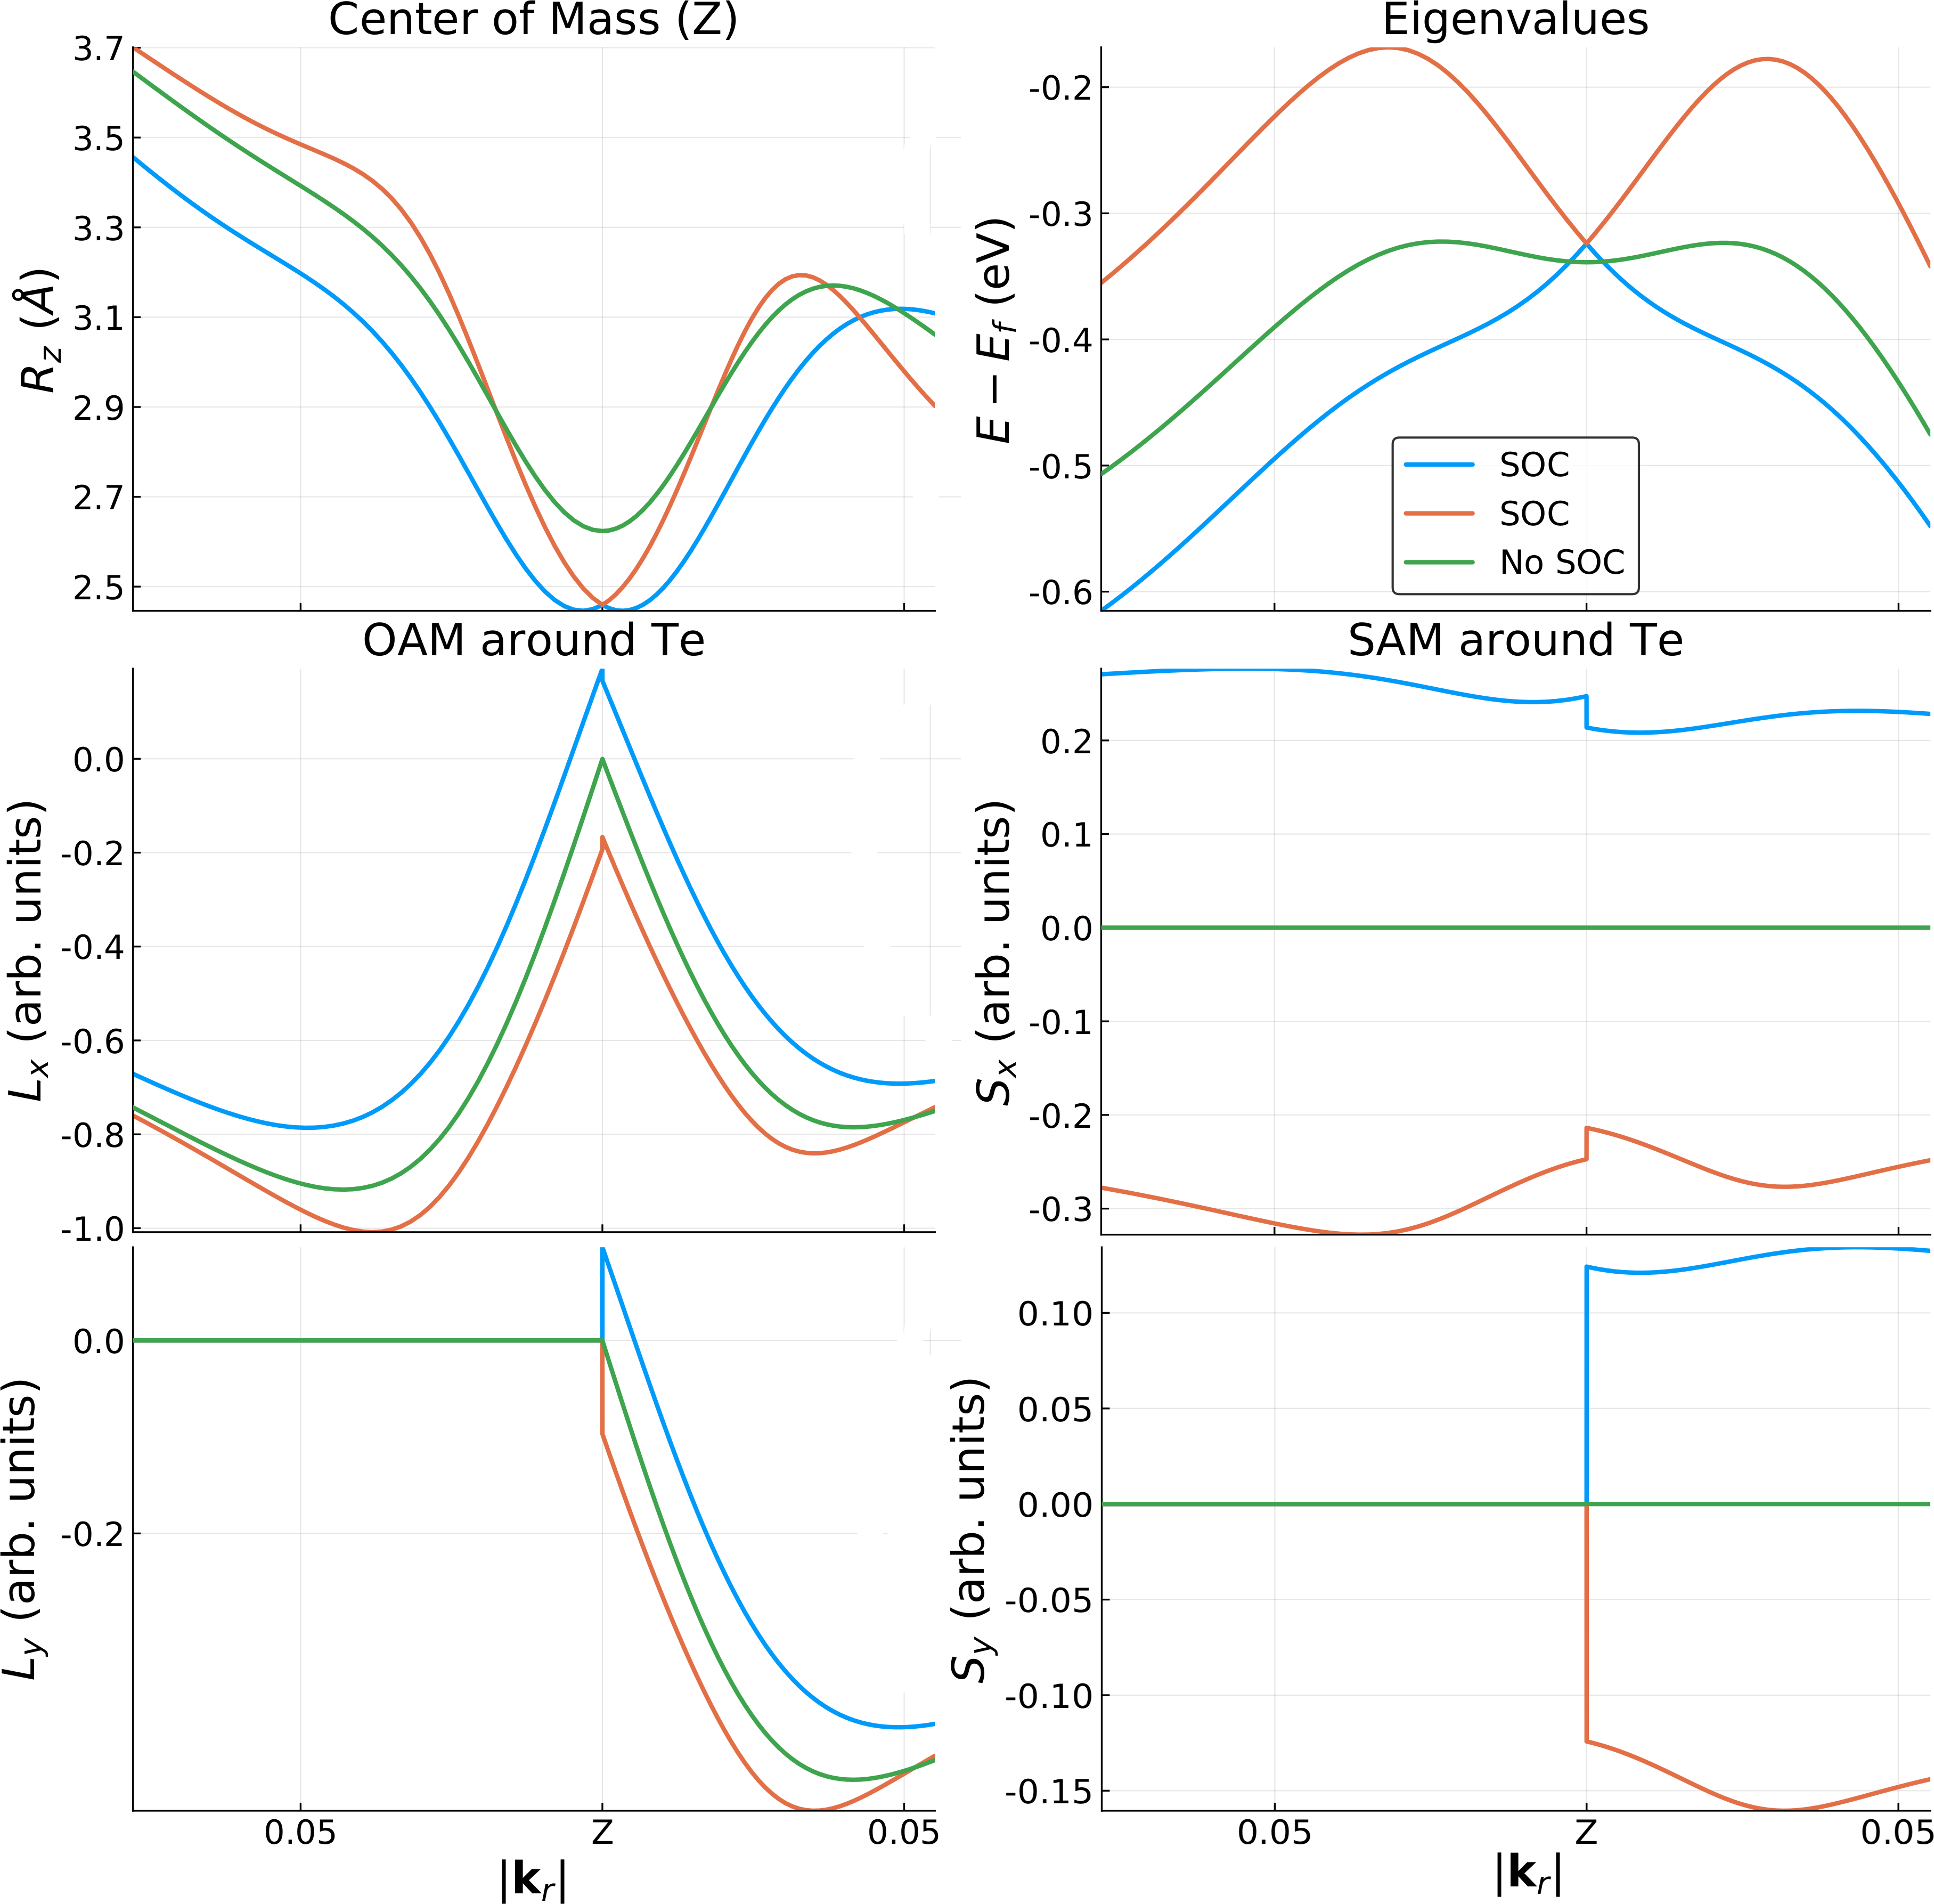
\includegraphics[width=\linewidth]{OAMvsK}
% \caption{}
% \end{subfigure}
% ~
% \begin{subfigure}[b]{0.49\textwidth}
% \centering
% 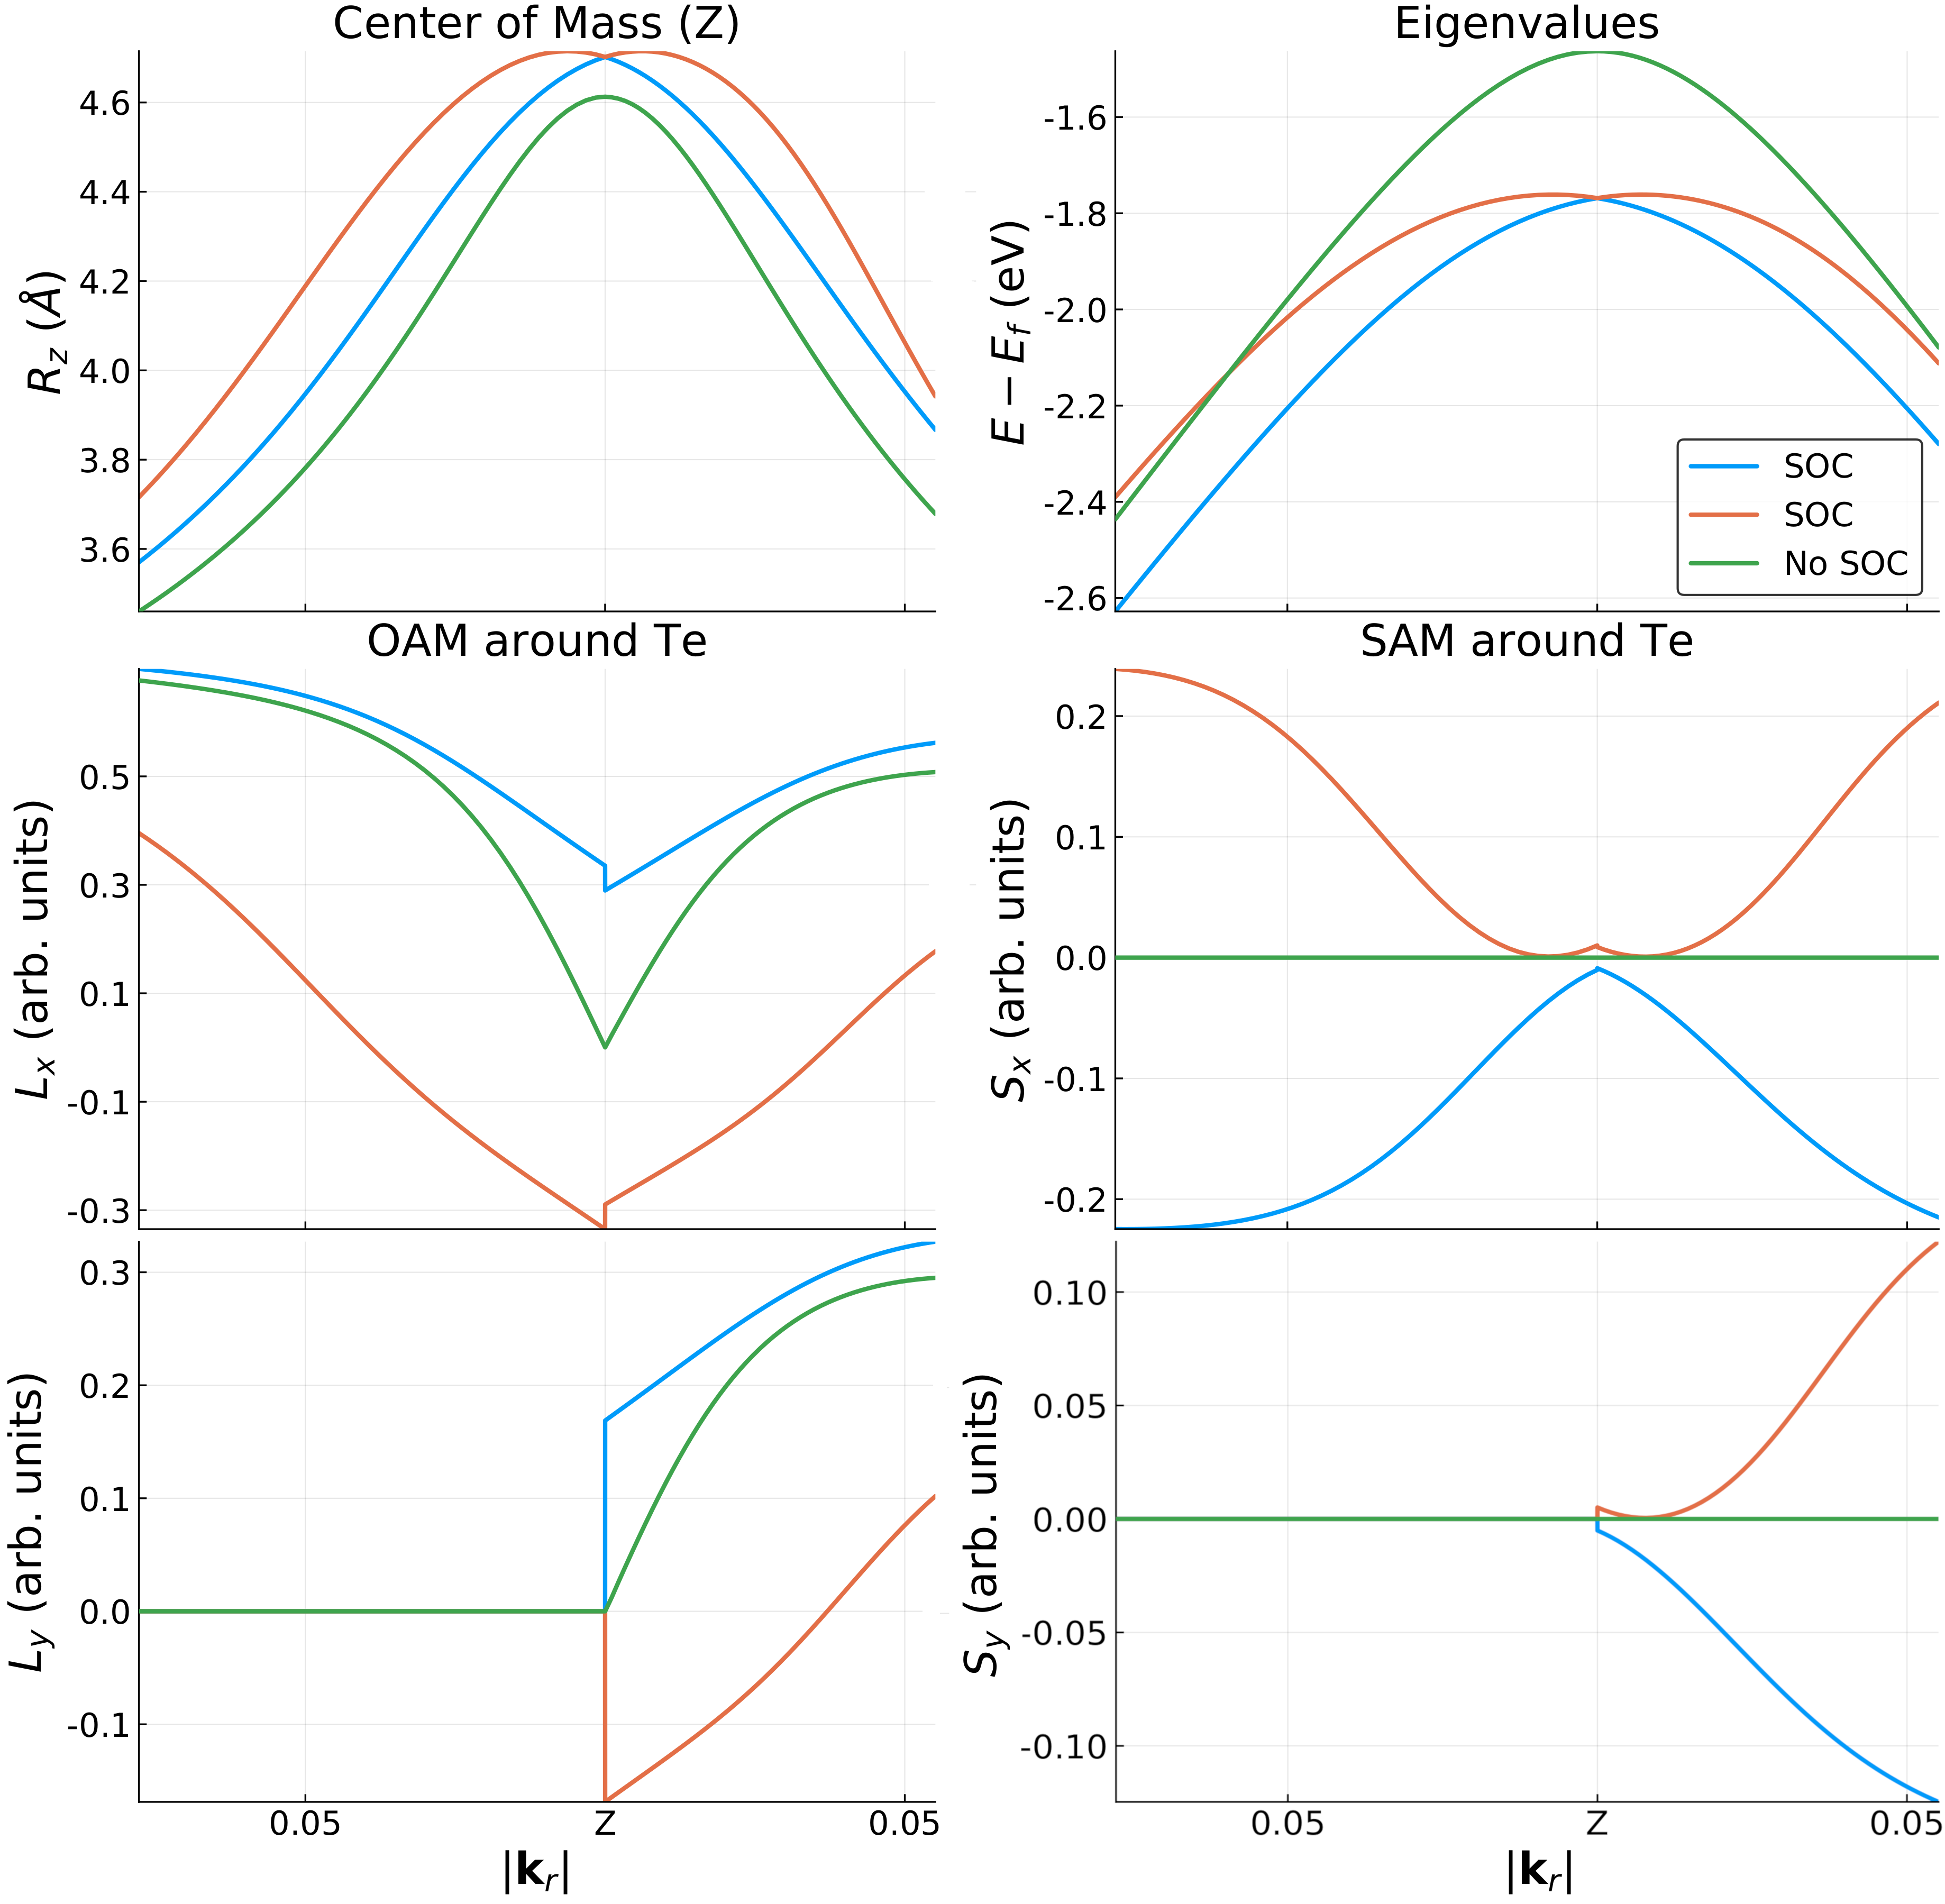
\includegraphics[width=\linewidth]{OAMvsK2.png}
% \caption{}
% \end{subfigure}
% %{oamvseigvalsv1.pdf}
% \caption{Comparison between the real-space observables and energy dispersion in (a) the first and (b) third valence band. The values are plotted in function of the relative distance from the $Z$ point $\bm{k}_r = \bm{k} - \bm{k}_Z$, towards the A and U points. The green graphs denote the values before turning on atomic SOC, whereas the orange and blue graphs denote the two spin-split bands.}\label{fig:oamvseigvalv}
% \end{figure*}
\begin{figure*}[ht!]
\centering
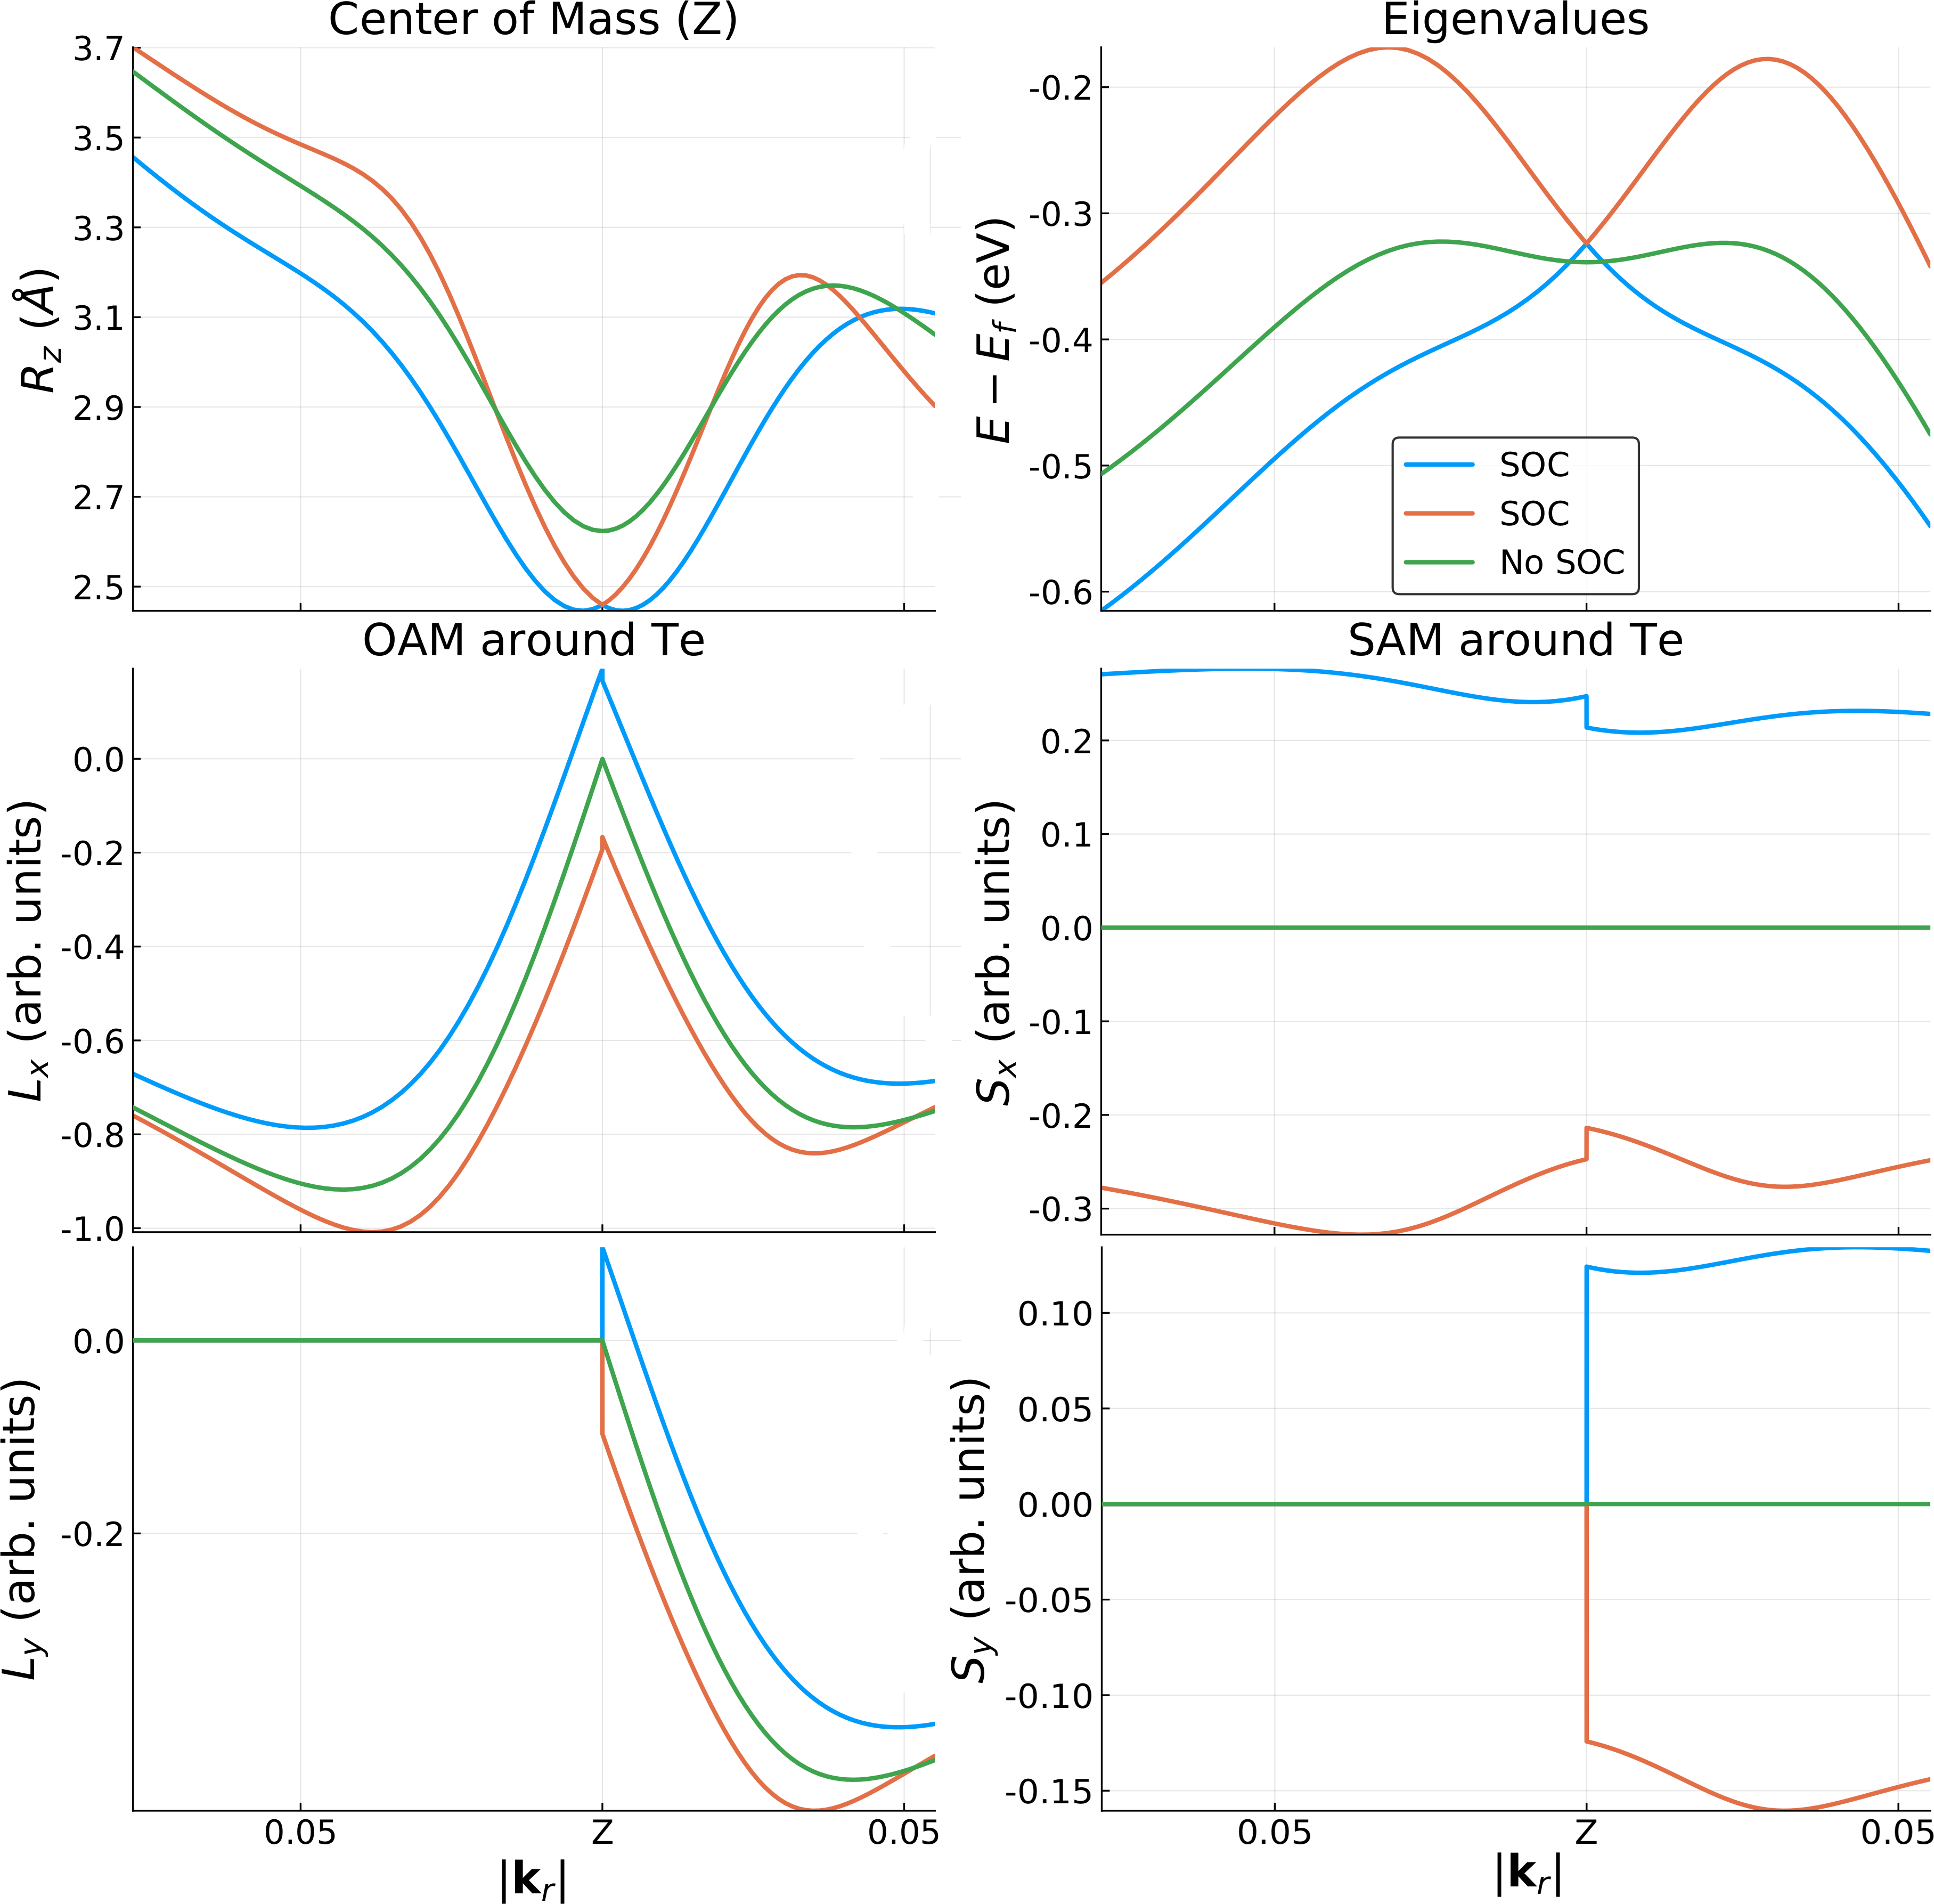
\includegraphics[width=0.49\linewidth]{OAMvsK}
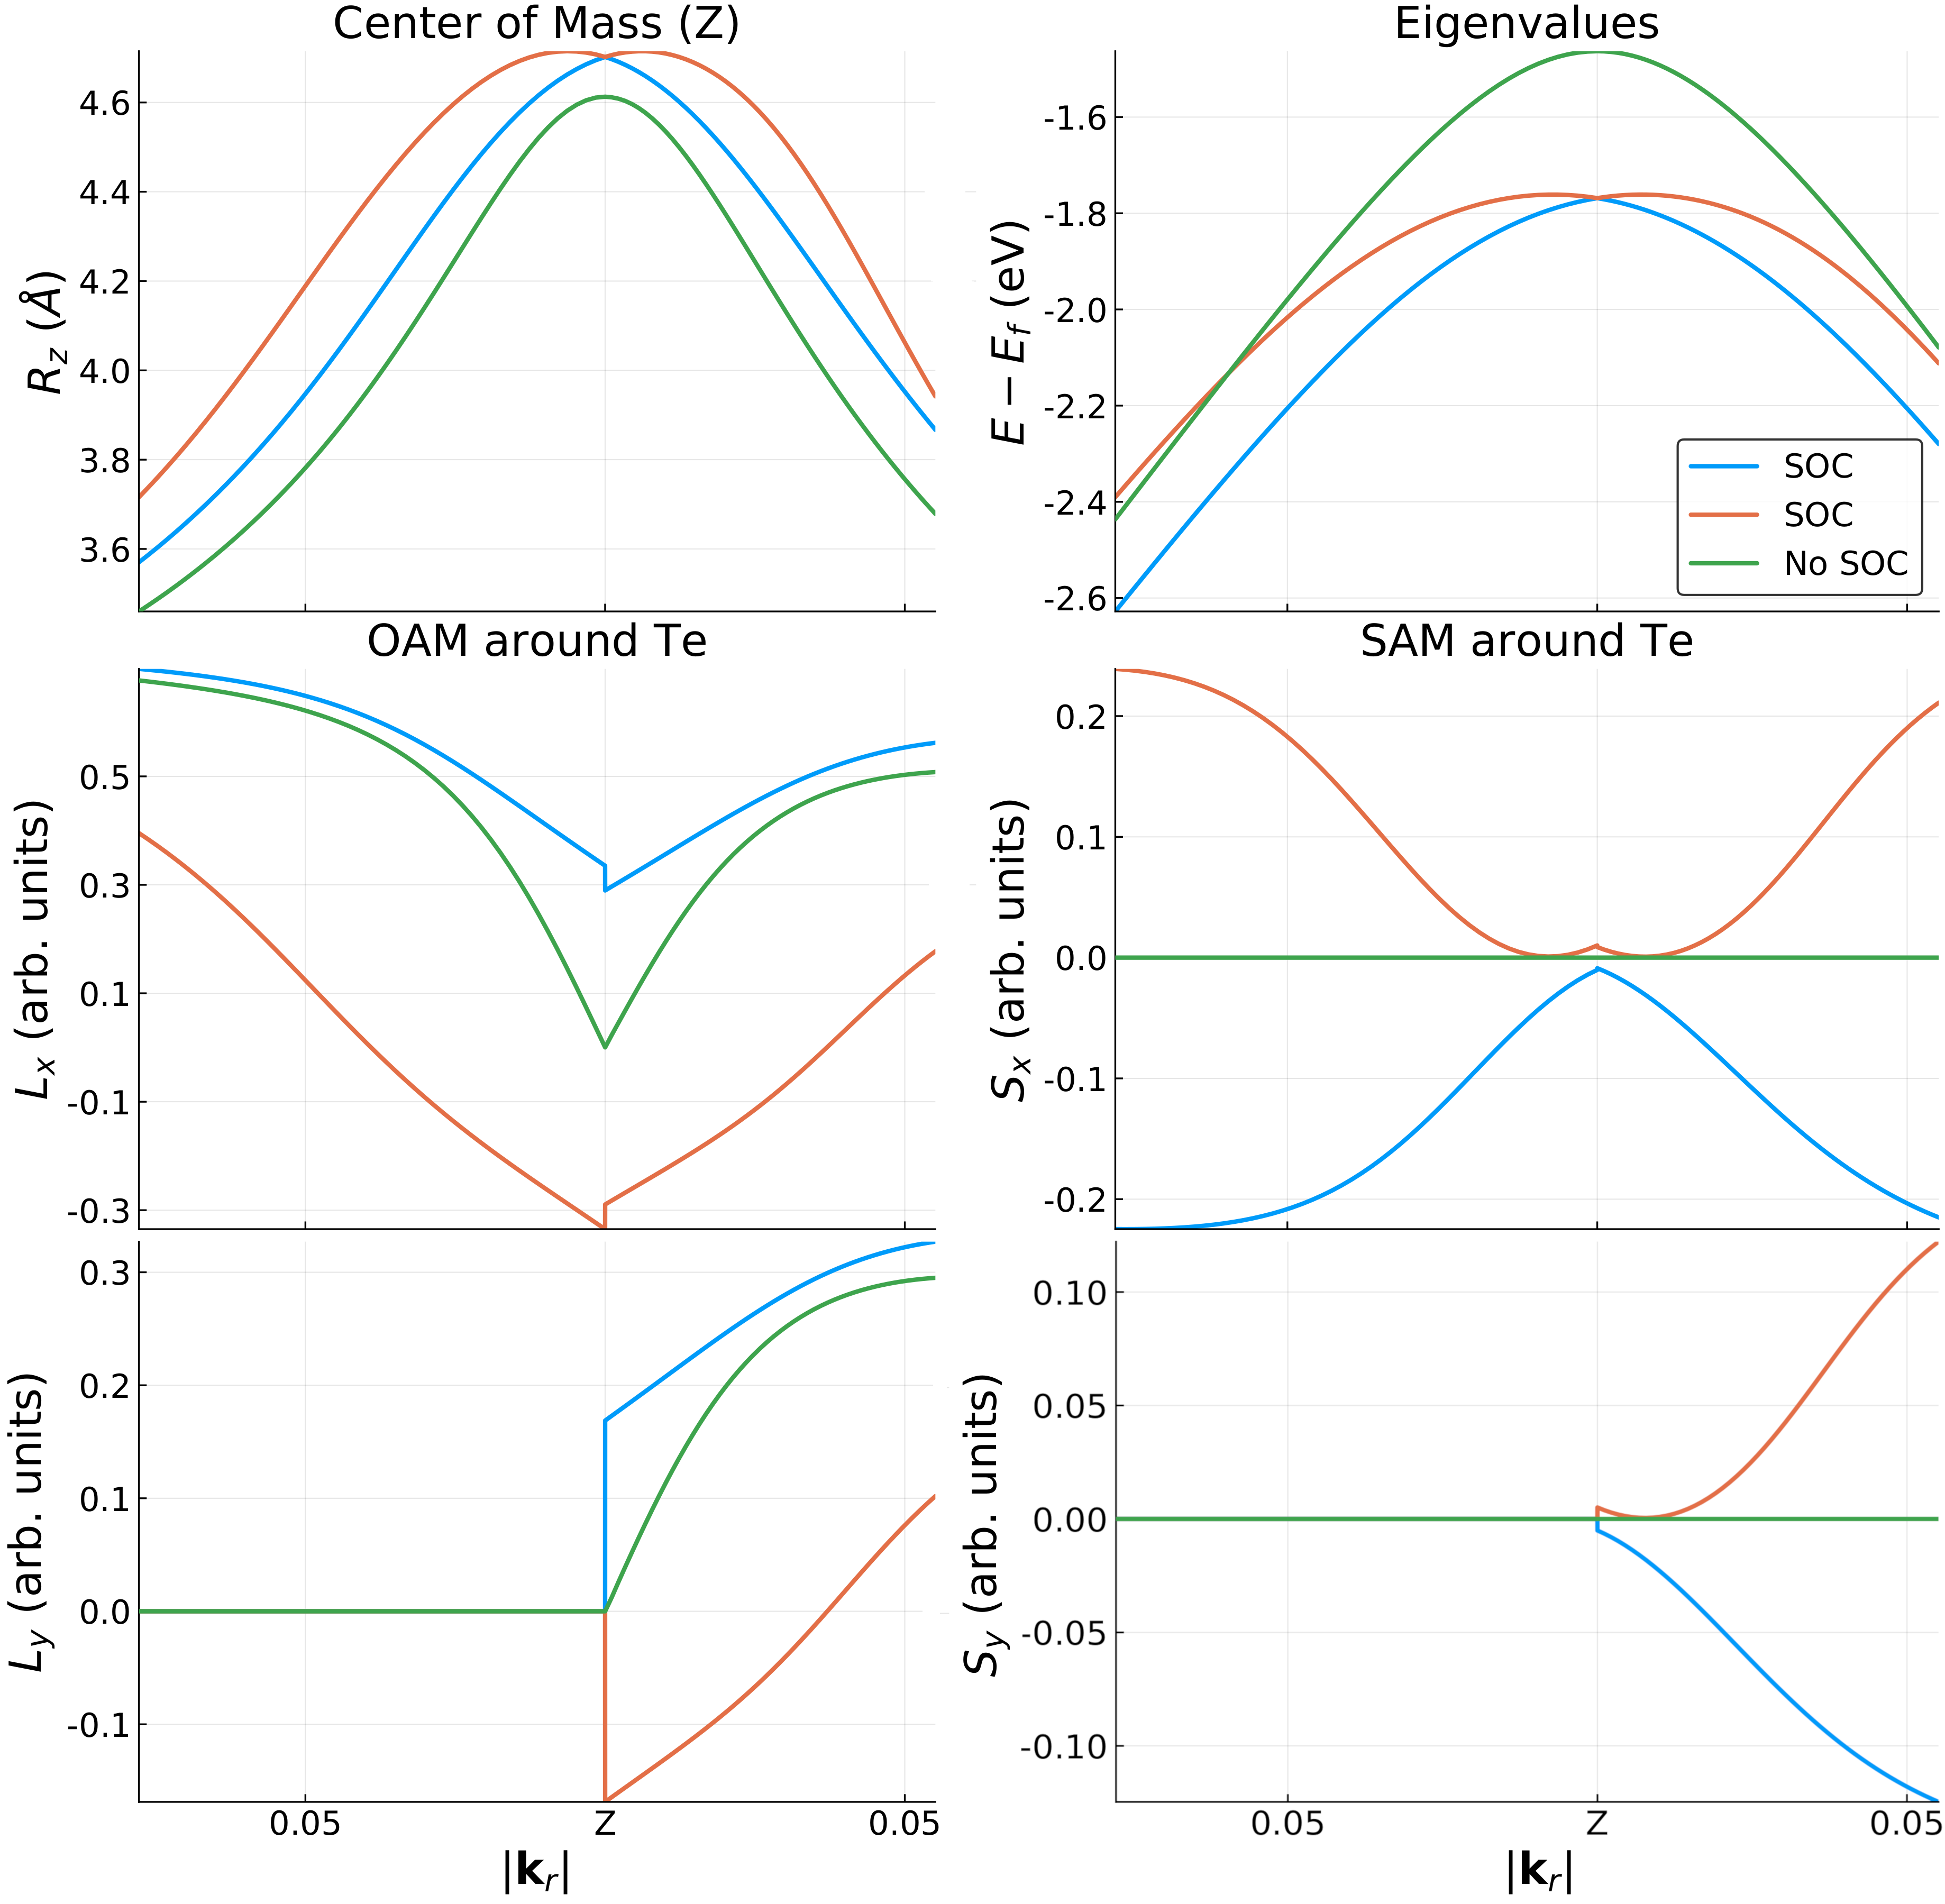
\includegraphics[width=0.49\linewidth]{OAMvsK2.png}
\caption{Comparison between the real-space observables and energy dispersion in (a) the first and (b) third valence band. The values are plotted in function of the relative distance from the $Z$ point $\bm{k}_r = \bm{k} - \bm{k}_Z$, towards the A and U points. The green graphs denote the values before turning on atomic SOC, whereas the orange and blue graphs denote the two spin-split bands.}\label{fig:oamvseigvalv}
\end{figure*}
Wannier representation allows us to elucidate the $k$-dependent electric dipole moment arising due to interference of the atomic orbitals on the neighboring sites \cite{Marzari2012MaximallyApplications}. In order to obtain the effective Hamiltonian, we write the Bloch functions as linear combinations of the Wannier functions that describe the bands of interest: $$\psi_{\bm{k}}(\bm{r})=\sum_{\alpha,\bm{R}} c_\alpha(\bm{k}) w_\alpha(\bm{r}-\bm{R})e^{i\bm{k}\bm{R}},$$ where the Wannier functions $w_\alpha(r)$ are chosen to be real and $\bm{R}$ denote the unit cell in which the orbital is centered.

In the case of GeTe the electric polarization is along the $z$ direction, making it sufficient to focus on the corresponding dipole moment
\begin{align}
d_z(\bm{k}) &=e\sum_{\alpha,\beta,\bm{R}}A_{\alpha,\beta}(\bm{k})e^{i\bm{k}.\bm{R}} \, \mathcal{Z}_{\alpha,\beta}^{\bm{R}} \\
A_{\alpha,\beta}(\bm{k}) &= c_{\alpha}^*(\bm{k}) c_\beta(\bm{k}) \\
\mathcal{Z}_{\alpha,\beta}^{\bm{R}} &= \int d\bm{r}   w_{\alpha}(\bm{r})w_\beta(\bm{r}-\bm{R}) z. \label{eq:Znn}
\end{align}
Expanding each term around $k_Z$, and keeping contributions up to first order in $\bm{k}^r = (k_Z - \bm{k})$, one obtains
\begin{align}\label{eq:dip}
d_z(\bm{k}) =e\sum_{\alpha,\beta,\bm{R}} &\left(A_{\alpha,\beta}(Z) + \bm{k}^r \left.\frac{\partial A_{\alpha,\beta}(\bm{k}) }{\partial \bm{k}}\right\rvert_{\bm{k}=Z}\right) \times \nonumber \\ 
&(1 + i\bm{k}^r \cdot \bm{R}) \mathcal{Z}_{\alpha,\beta}^{\bm{R}}.
\end{align}
The term that combines the first order variation of $A_{\alpha,\beta}(\bm{k})$ with the zeroth order term from the exponent leads to a nonzero contribution only if $w_\alpha, w_\beta = s, p_z$ in the same unit cell ($\bm{R}=0$).
This is the charge asymmetry that comes from $s$-$p_z$ hybridization and was previously considered in the context of giant spin splitting at surfaces in Refs.~\citenum{Petersen2000SimpleStates,Go2016SurfacePhysics} and for bulk perovskites in Ref.~\citenum{Kim2014}.
The new terms that we consider here combine the zeroth and first order contributions to $A_{\alpha,\beta}(\bm{k})$ with the first order $i\bm{k}^r \cdot \bm{R}$ term.
Using indices $1,2,3$ to denote $p_x, p_y, p_z$ Wannier functions one obtains the following relation between the Bloch function coefficients and the OAM: $l_k(\bm{k}) = -i \epsilon_{ijk} A_{ij}$.%\sa{only for pure $p_x$ etc. functions}

% \begin{figure}[t]
% ~\centering
% 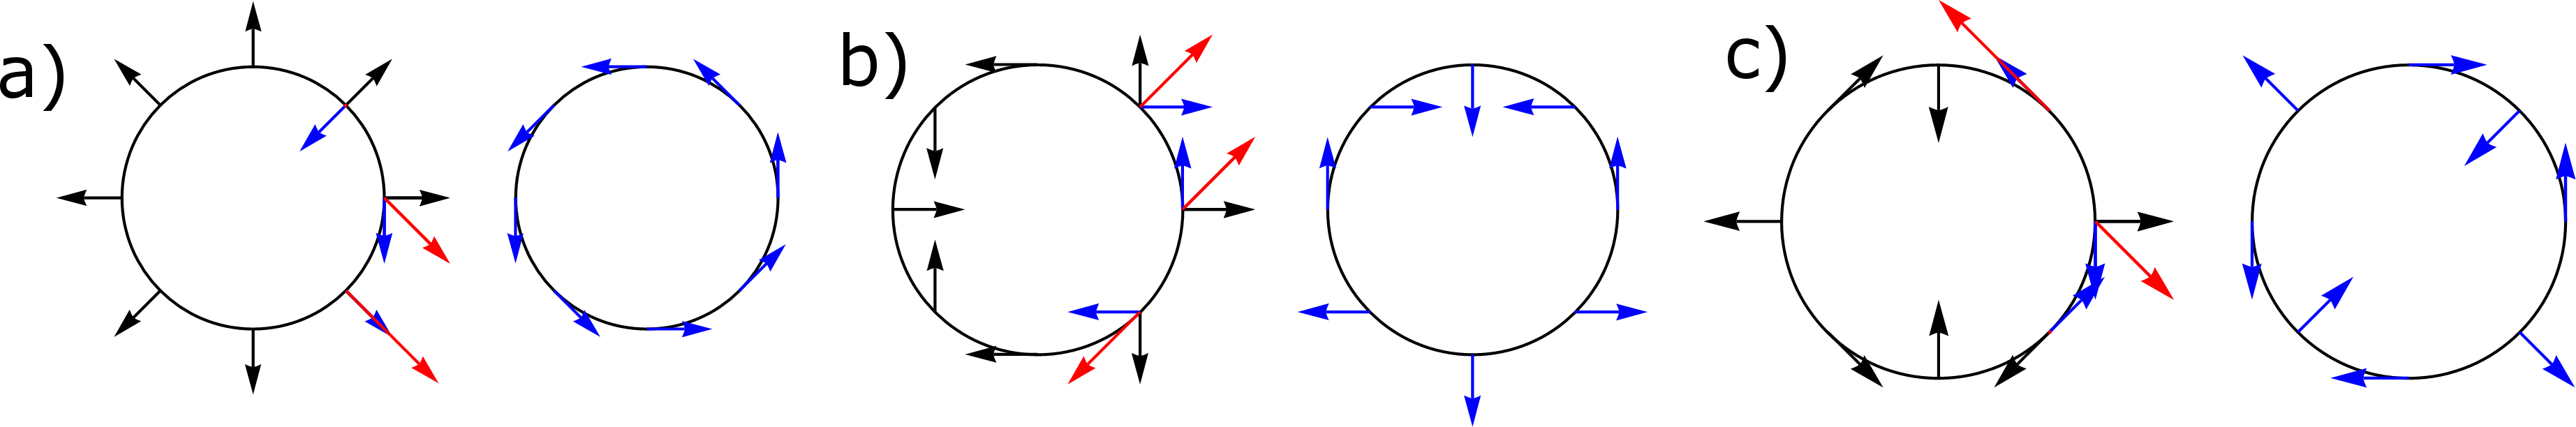
\includegraphics[width=\linewidth]{1_1.png}\caption{\label{fig:overlaparrows} Dipoles due to interference for $p$, $d$ and $f$ orbitals, with maximal angular momentum projection, $\psi\sim e^{i l\phi}$, are shown in panels (a) - c) respectively. Black and blue arrows denote the complex phases of wavefunctions in neighboring unit cells, where the red arrow shows the resulting complex amplitude of the total Bloch function due to interference of the orbitals. The overlapping orbitals where spaced apart for visual clarity.}
% \end{figure}
Upon closer inspection of the overlap dipole, $\mathcal{Z}_{\alpha,\beta}^{\bm{R}}$, one concludes that for $d_z$ to be nonzero, at least one of the orbitals $\alpha,\beta$ needs to be the $p_z$ orbital and the shift-vector $\bm{R}$ has to have a component along the second orbital ($p_x$ or $p_y$). This is illustrated in Fig.~\ref{fig:overlapdip}(a). 
% Another requirement for this term to be nonzero is that the orbitals have odd parity, such as $p$ and $f$. This is highlighted in Fig.~\ref{fig:overlaparrows}. If they have even parity (as is the case for the $d$ orbitals displayed in Fig.~\ref{fig:overlapdip}(b) and ~\ref{fig:overlaparrows}(b)), the overlap dipoles from neighboring unit cells will cancel. 
Filling this into Eq.~(\ref{eq:dip}) and summing over the nearest neighbor unit cells ($\bm{R} = \pm 1$), we arrive at
\begin{align}\label{eq:dipfinal}
    d_z(\bm{k}) &= 4e \left(l_x(Z) + \bm{k}^r \left.\frac{\partial l_x(\bm{k}) }{\partial \bm{k}}\right\rvert_{\bm{k}=Z}\right) k^r_yR_y \mathcal{Z}_{y,z}^{R_y}\nonumber \\
    &  - 4e\left(l_y(Z) + \bm{k}^r \left.\frac{\partial l_y(\bm{k}) }{\partial \bm{k}}\right\rvert_{\bm{k}=Z}\right) k^r_xR_x \mathcal{Z}_{x,z}^{R_x}.
\end{align}
The coupling of the electric dipole moment with an external electric field, or in the case of GeTe, with the electric polarization, leads to a contribution to the Hamiltonian of the form:
\begin{equation}\label{HOR}
    \mathcal{H}_{OR} \propto \bm{l} \cdot ( \bm{k} \times \bm{E})
\end{equation}
The terms with $l_{x,y}(Z)$ lead to a linear $k$-dependence of the band energy if the atomic SOC partially unquenches the OAM.
The second term leads to energy contribution, quadratic in $k$, but results in a linear variation of the OAM even in the absence of SOC. This linear variation of the OAM will then couple to $\bm{\sigma}$ [also referred to as spin angular momentum (SAM)] through the atomic SOC, leading to the linear spin splitting.

The energy dispersion close to the $Z$ point can thus be modeled by
\begin{equation}\label{eq:hami}
\epsilon(\bm{k}) = \epsilon(Z) + \lambda_{so} \bm{l}\cdot \bm{\sigma} + c_1 \bm{l} \cdot ( \bm{k} \times \bm{E})+ c_2 l_z^2,
\end{equation}
where $\epsilon(Z)$ contains a constant band shift, while the term with $\lambda$ is the atomic spin-orbit coupling, and the latter terms represent the contribution due to the threefold symmetric crystal field for $l=1$.
To explicitly show how the linear variation of the OAM arises from the terms in Eq.~(\ref{eq:dipfinal}), we performed a $k\cdot p$-expansion of the first valence band which leads to following expressions for the OAM around $k=Z$:
\begin{align}\label{eq:OAM}
l_x &= -\frac{\lambda_{so}\sigma_x - c_1 E_z k_y}{c_2} \\
l_y &= -\frac{\lambda_{so}\sigma_y + c_1 E_z k_x}{c_2},\nonumber
\end{align}
where we only included terms with the $E_z$ component.
\begin{figure}
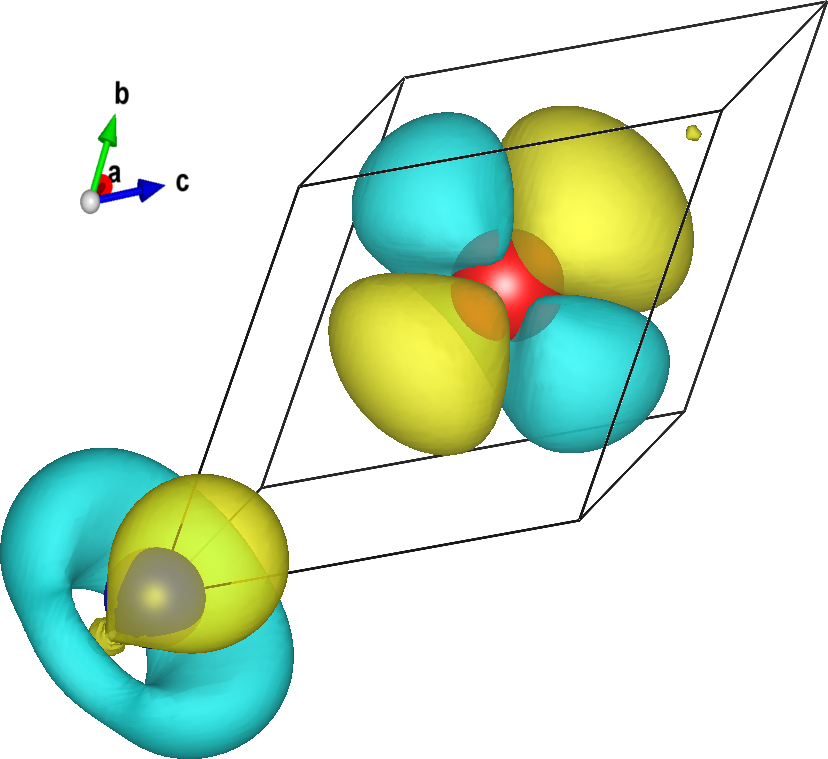
\includegraphics[width=.7\columnwidth]{diffdens}
\caption{\label{Fig:diffdens}The variation of the charge density of the Bloch function of the first valence band $\left.\frac{\partial |\psi(k)|^2}{\partial k}\right\rvert_{k=Z}$ away from $Z$ towards $A$. Te and Ge ions are in red and blue, respectively. The charge asymmetry around Ge showcases the nonzero dipole moment along $z$, which couples to the local electric field near Ge ion.}
\end{figure}
\begin{figure*}[t!]
  \subfloat[Lower 3rd valence band]{
    \centering
    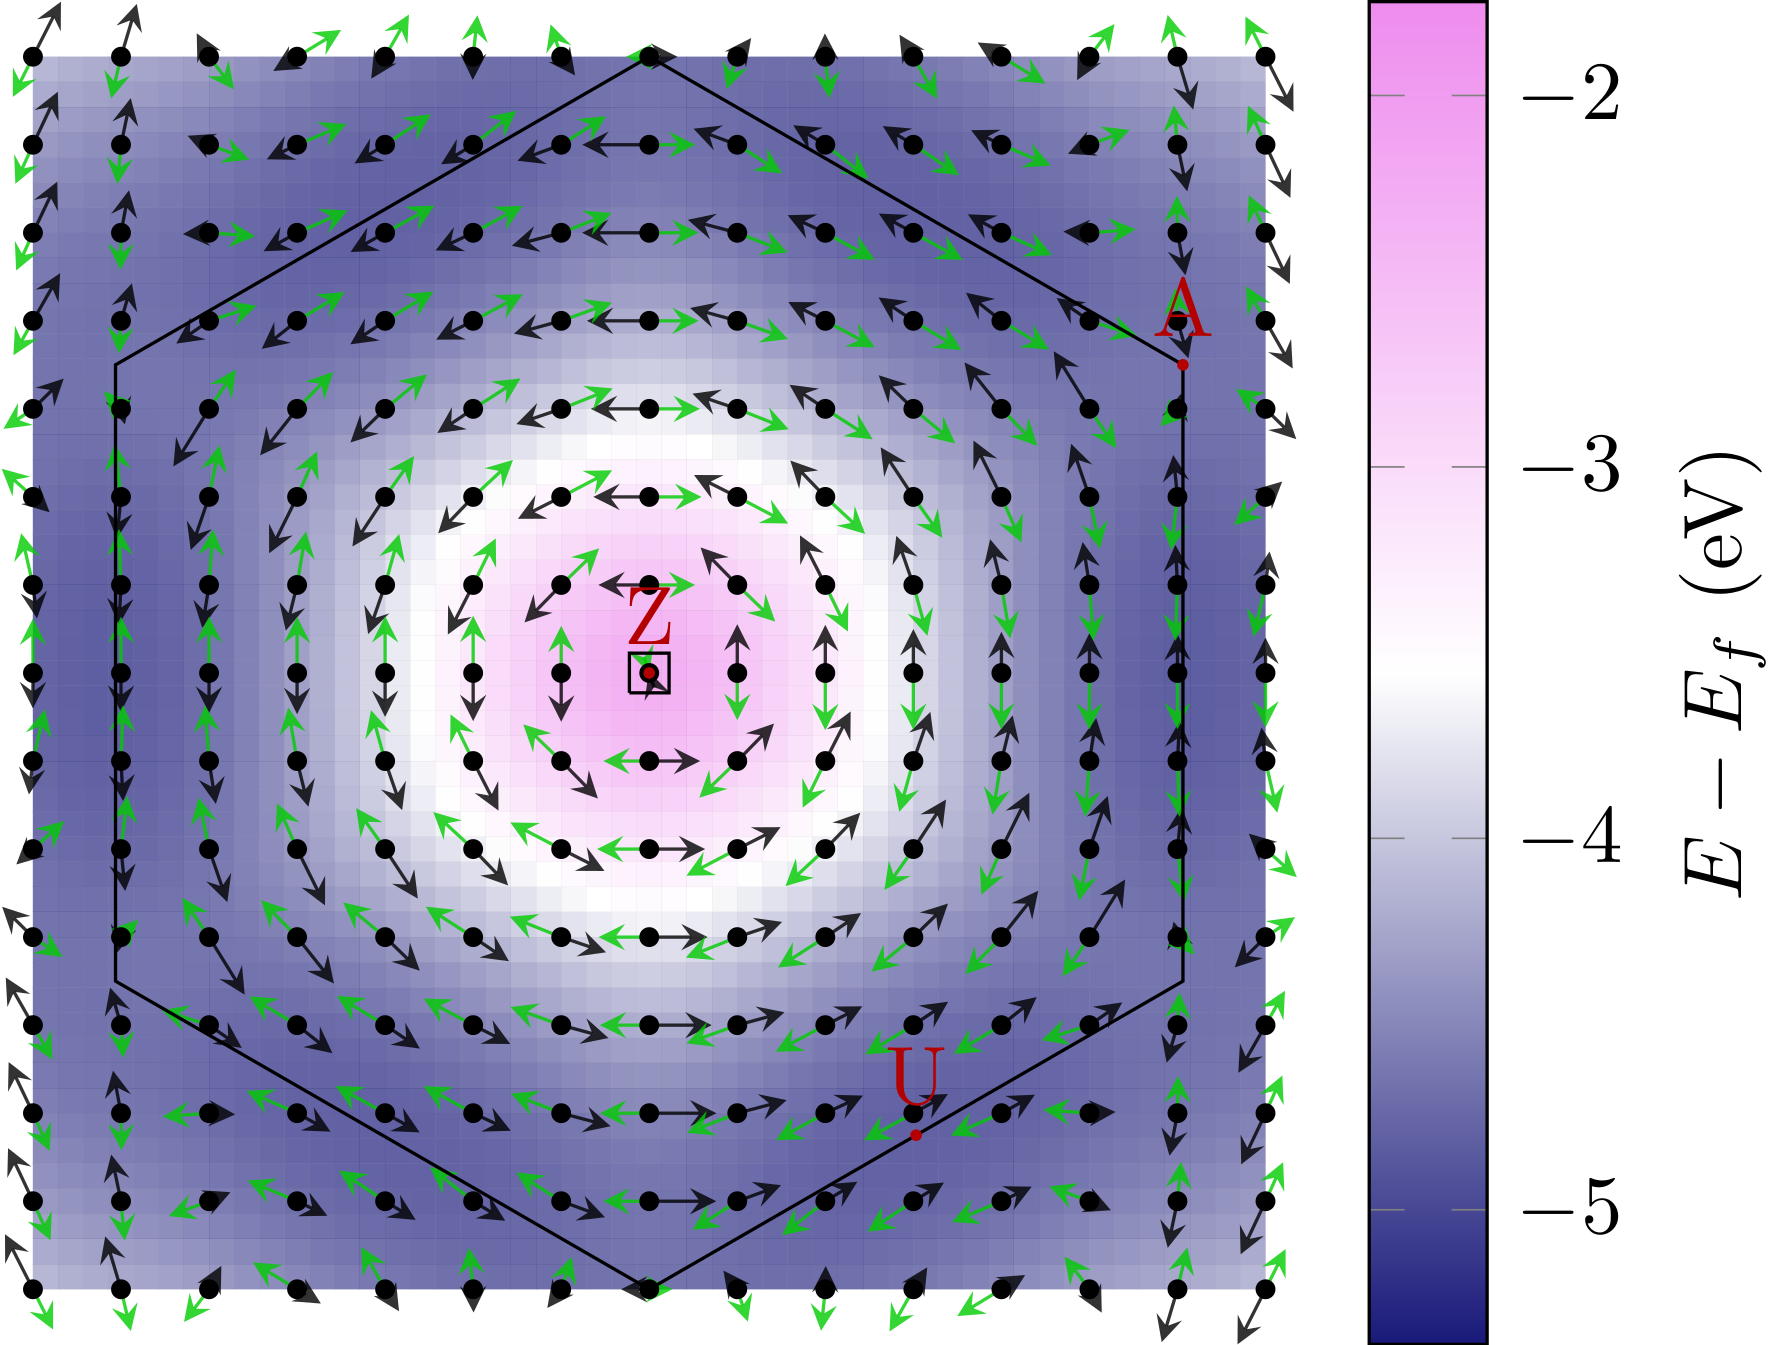
\includegraphics[width=0.32\linewidth]{Ltexture5.png}
  }
  ~
  \subfloat[Upper 3rd valence band]{
    \centering
    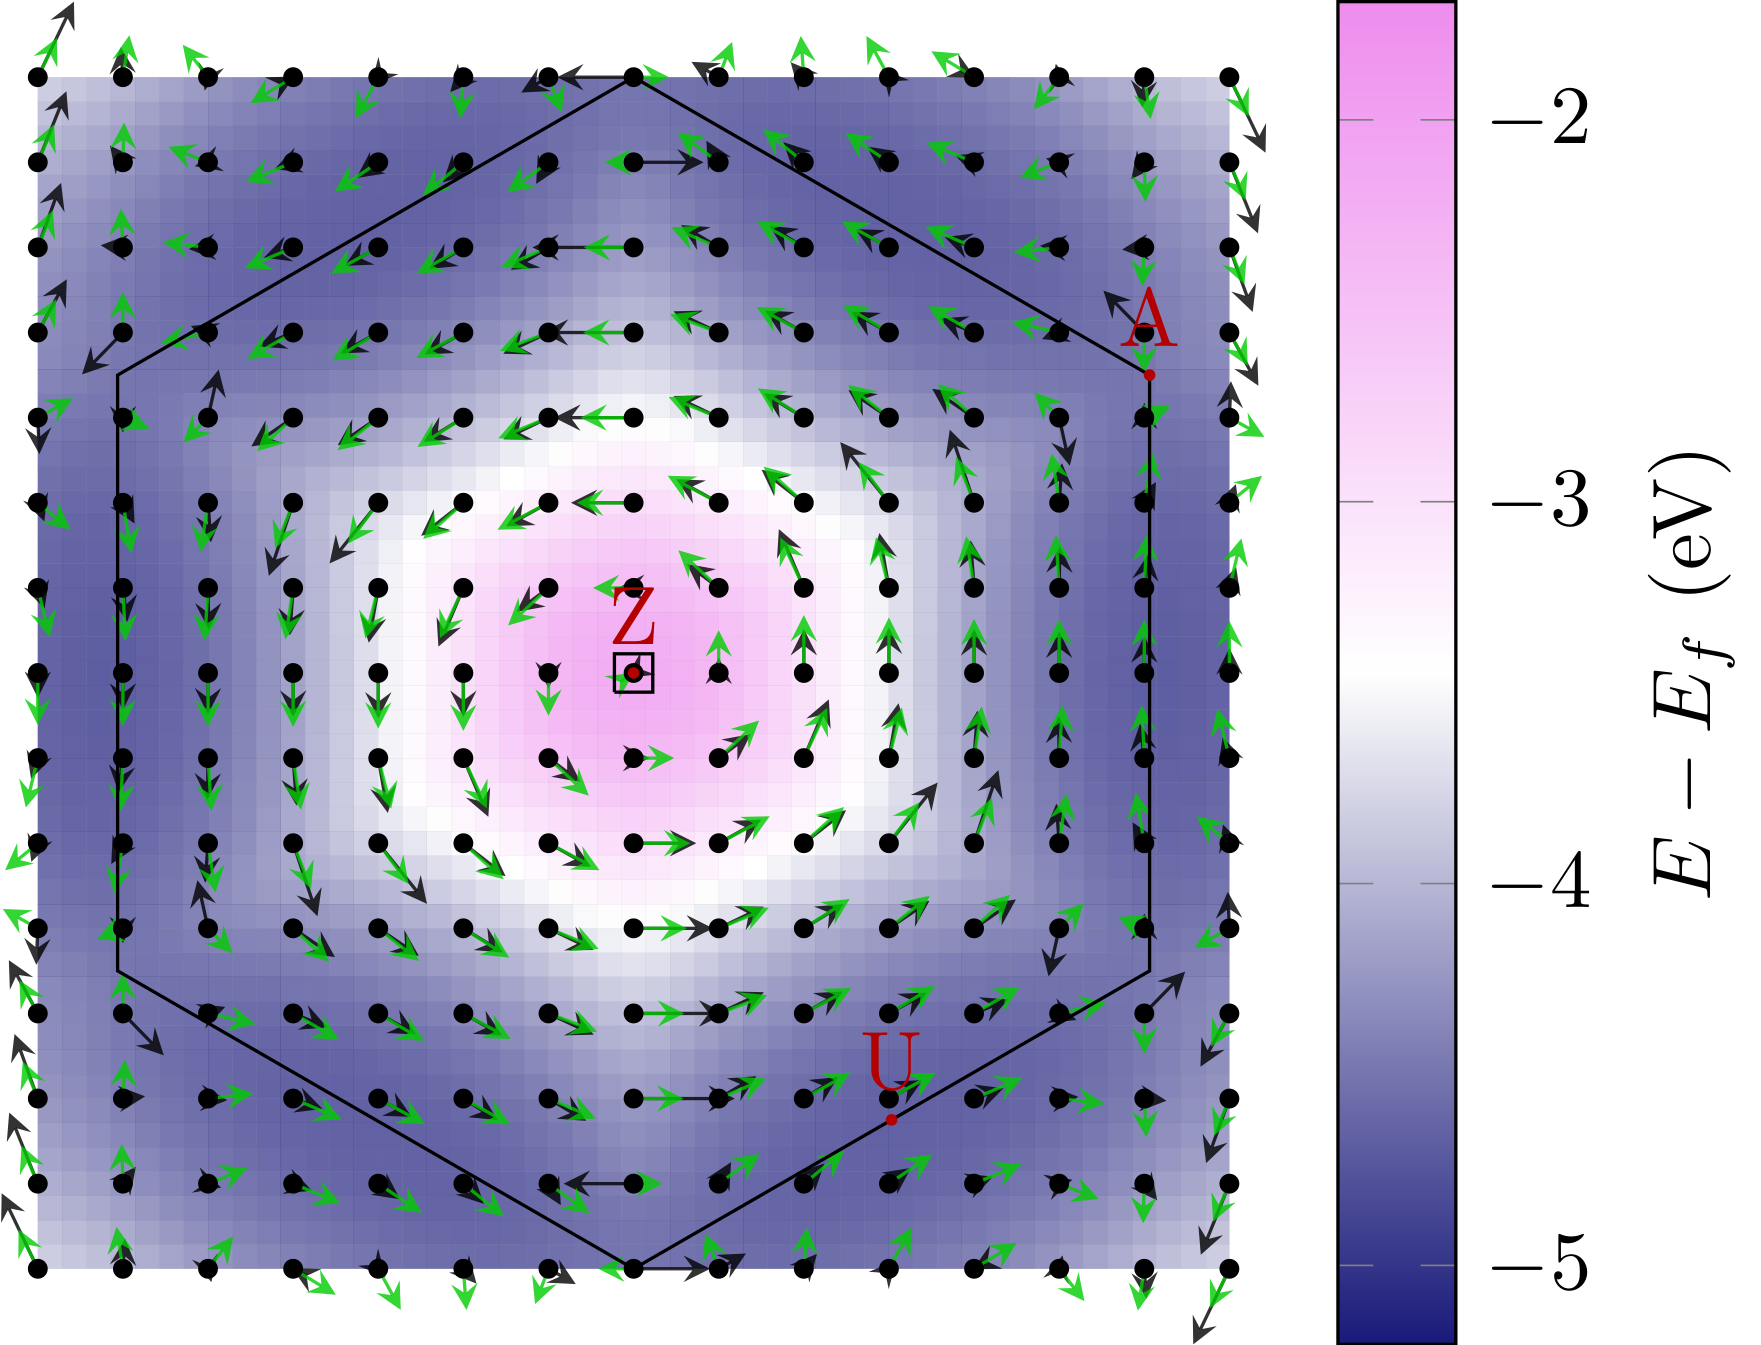
\includegraphics[width=0.32\linewidth]{Ltexture6.png}
  }
  ~
  \subfloat[Zoom-in of (b)]{
    \centering
    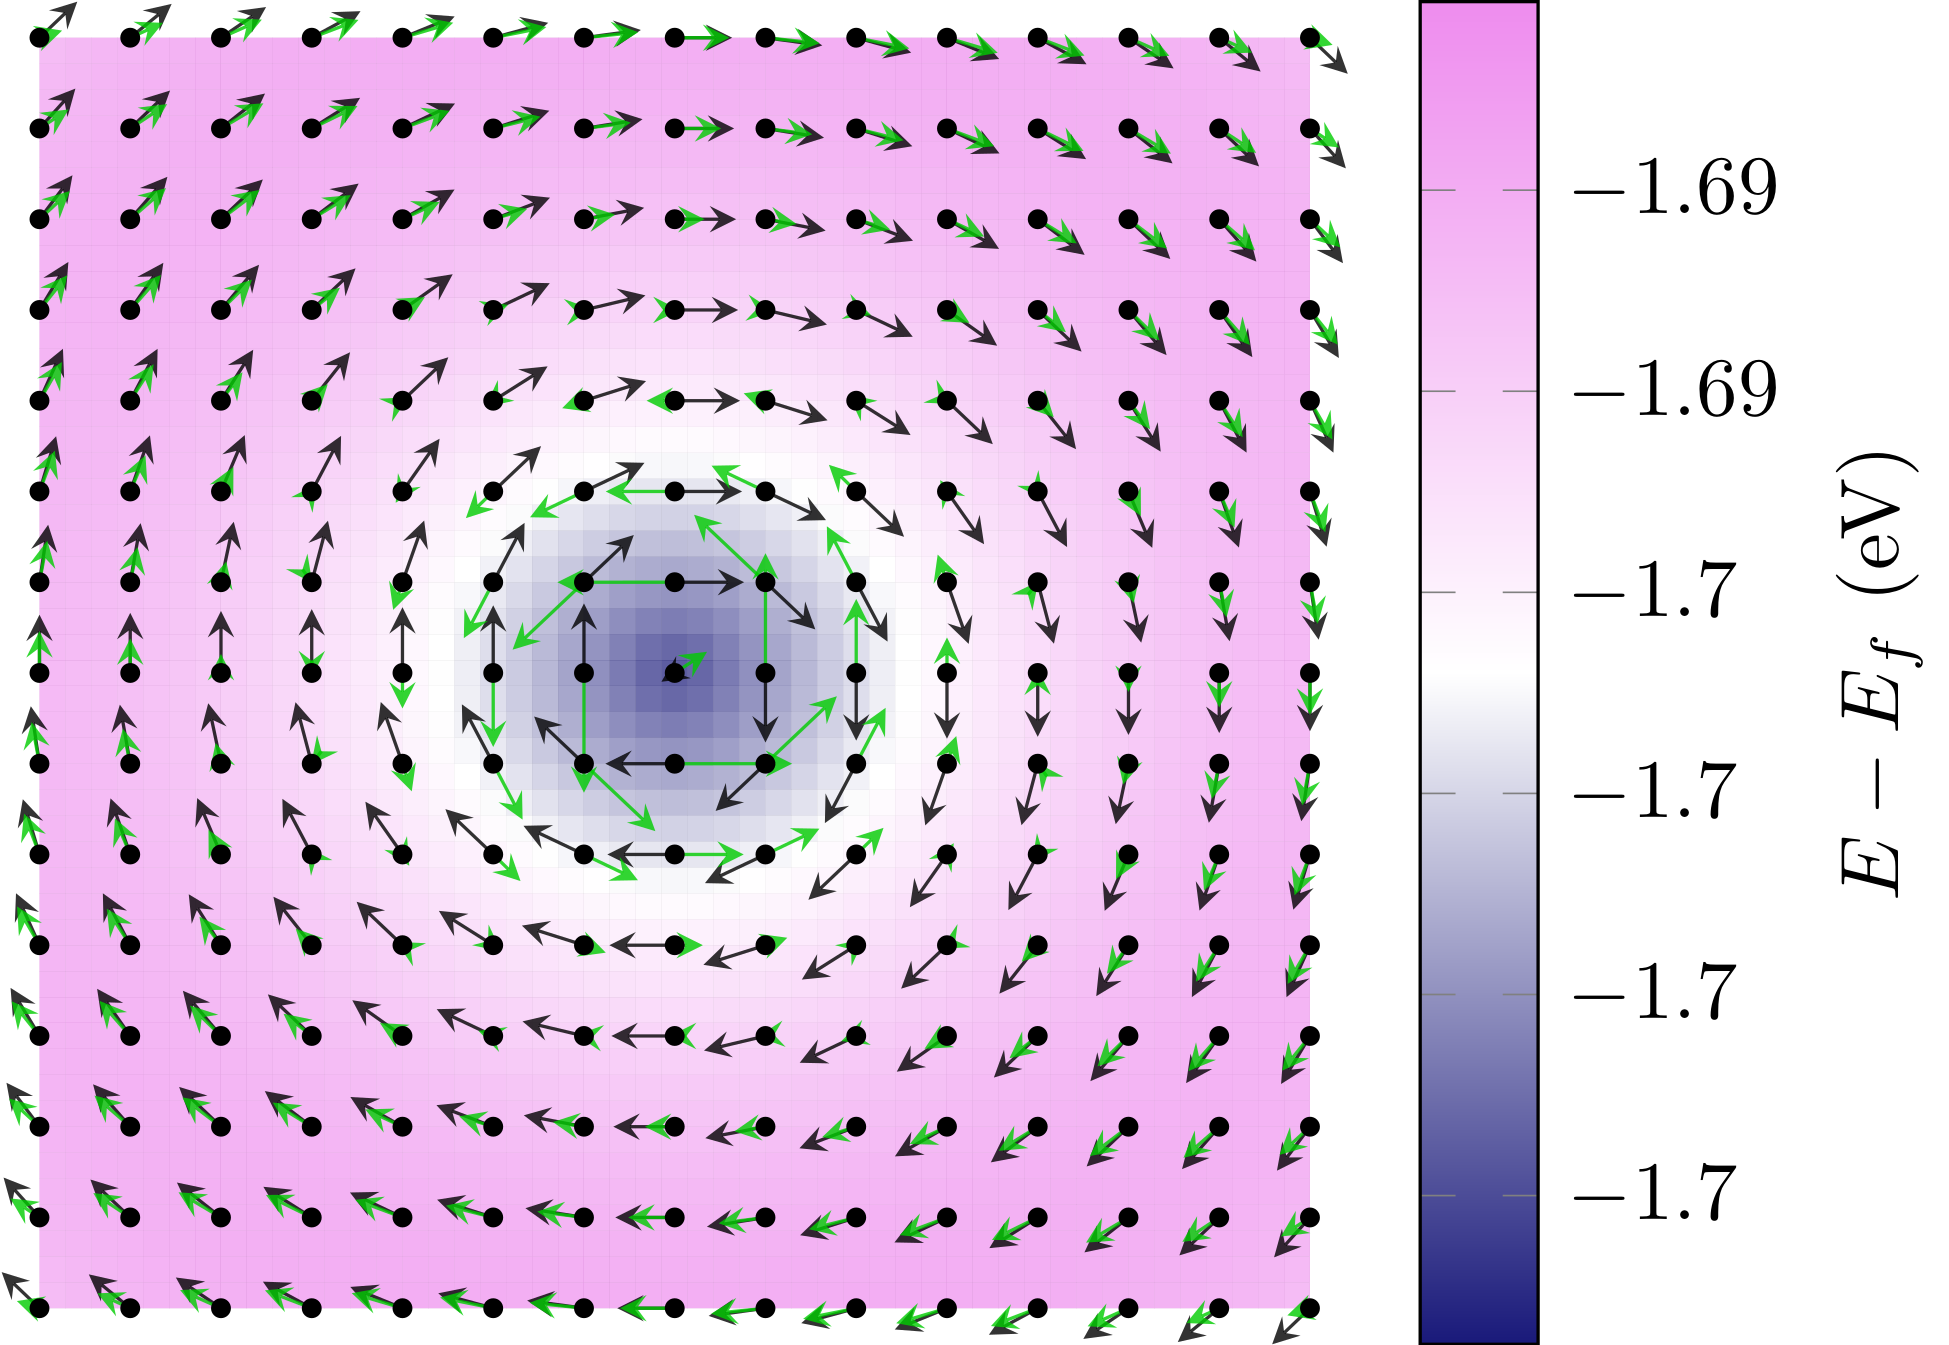
\includegraphics[width=0.34\linewidth]{Ltexture6small.png}
  }\\
  ~
  \subfloat[Lower 1st valence band]{
    \centering
    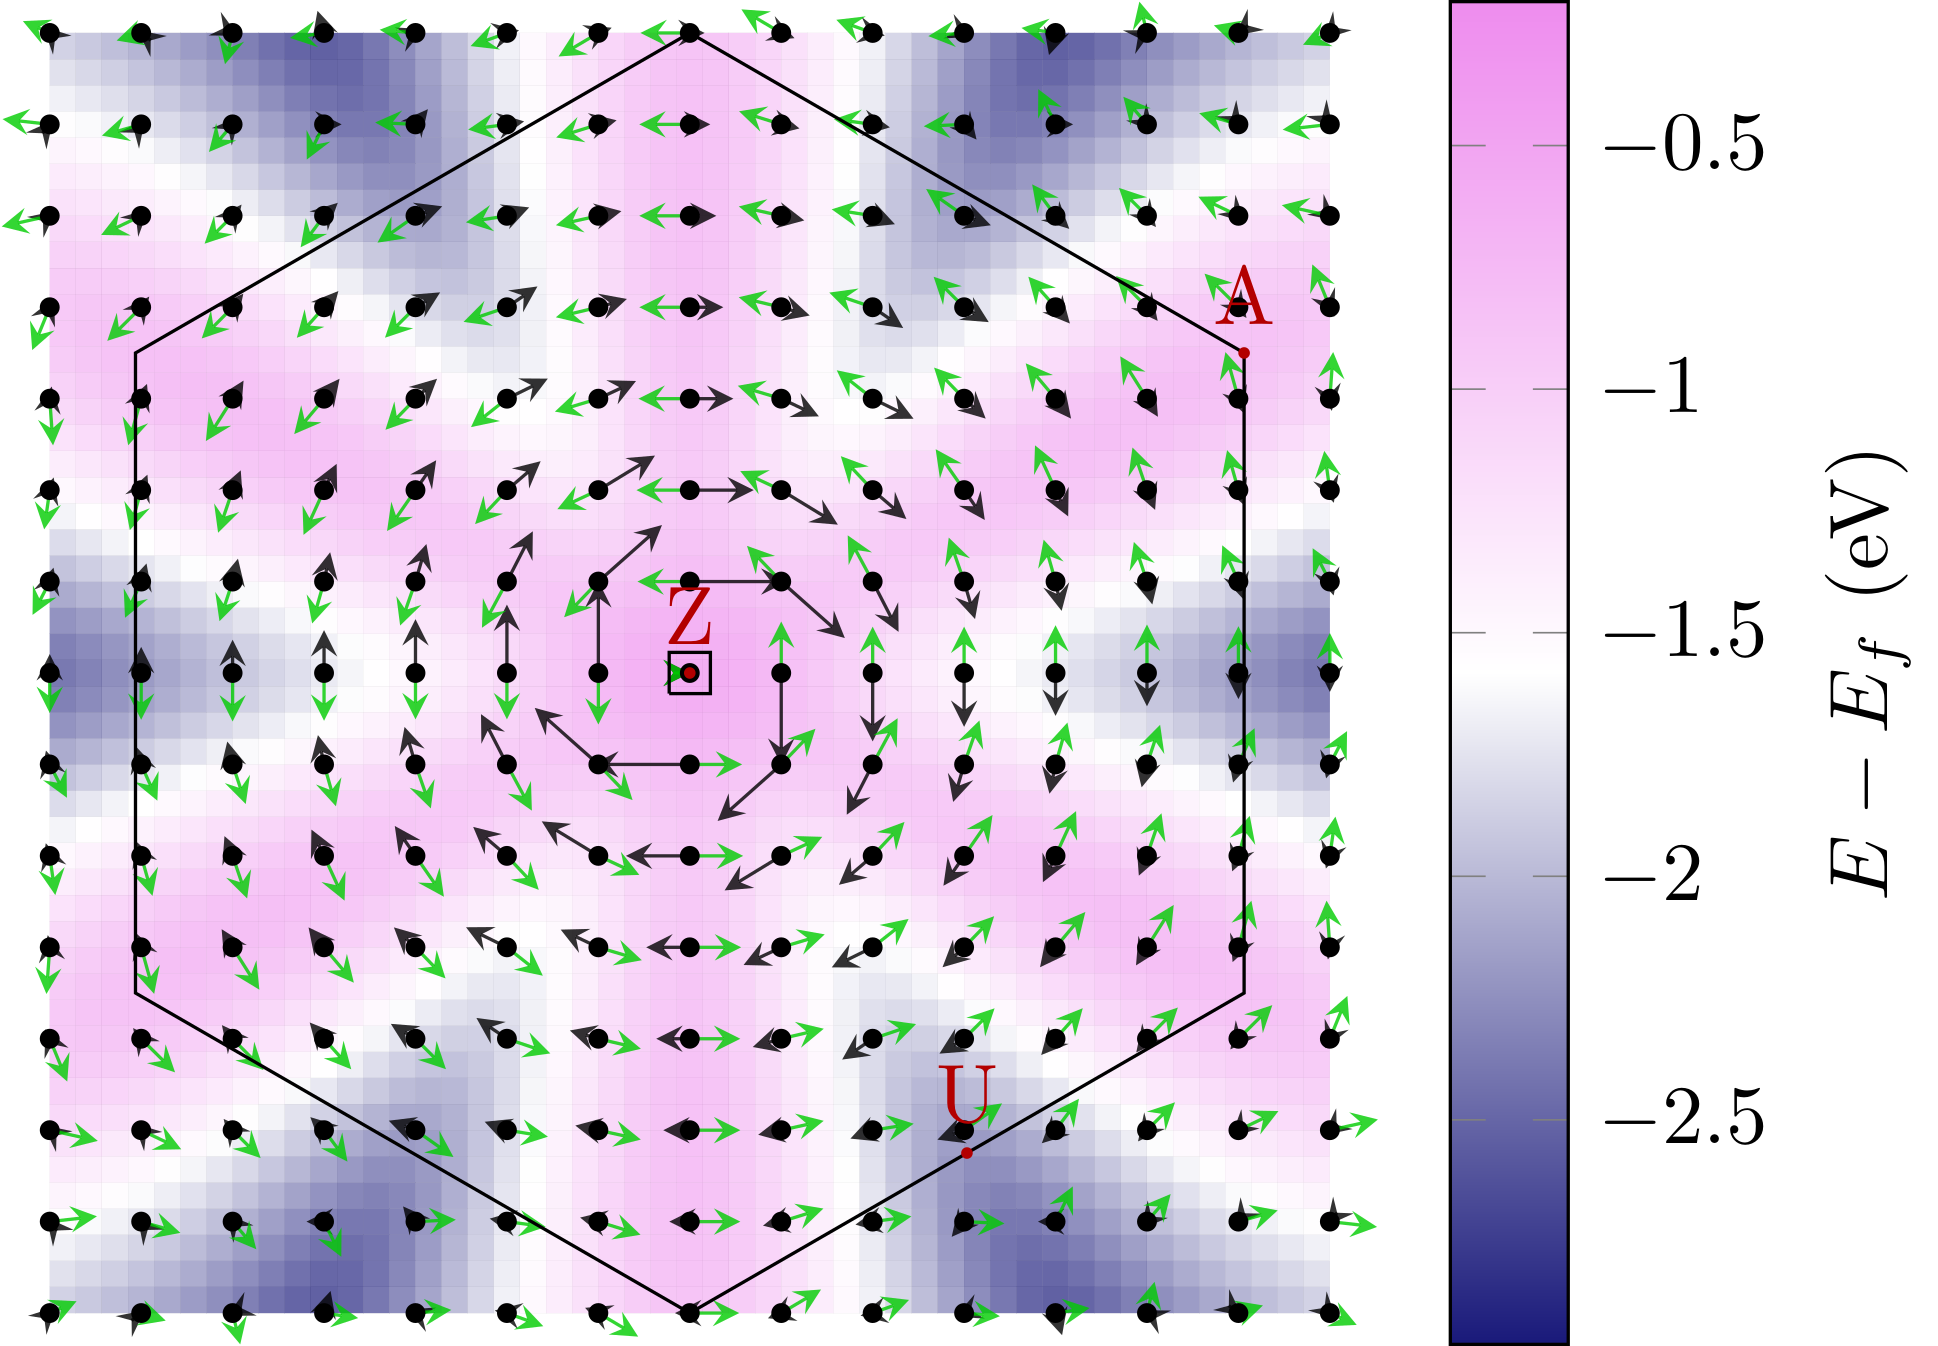
\includegraphics[width=0.32\linewidth]{Ltexture9.png}
  }
  ~
  \subfloat[Upper 1st valence band]{
    \centering
    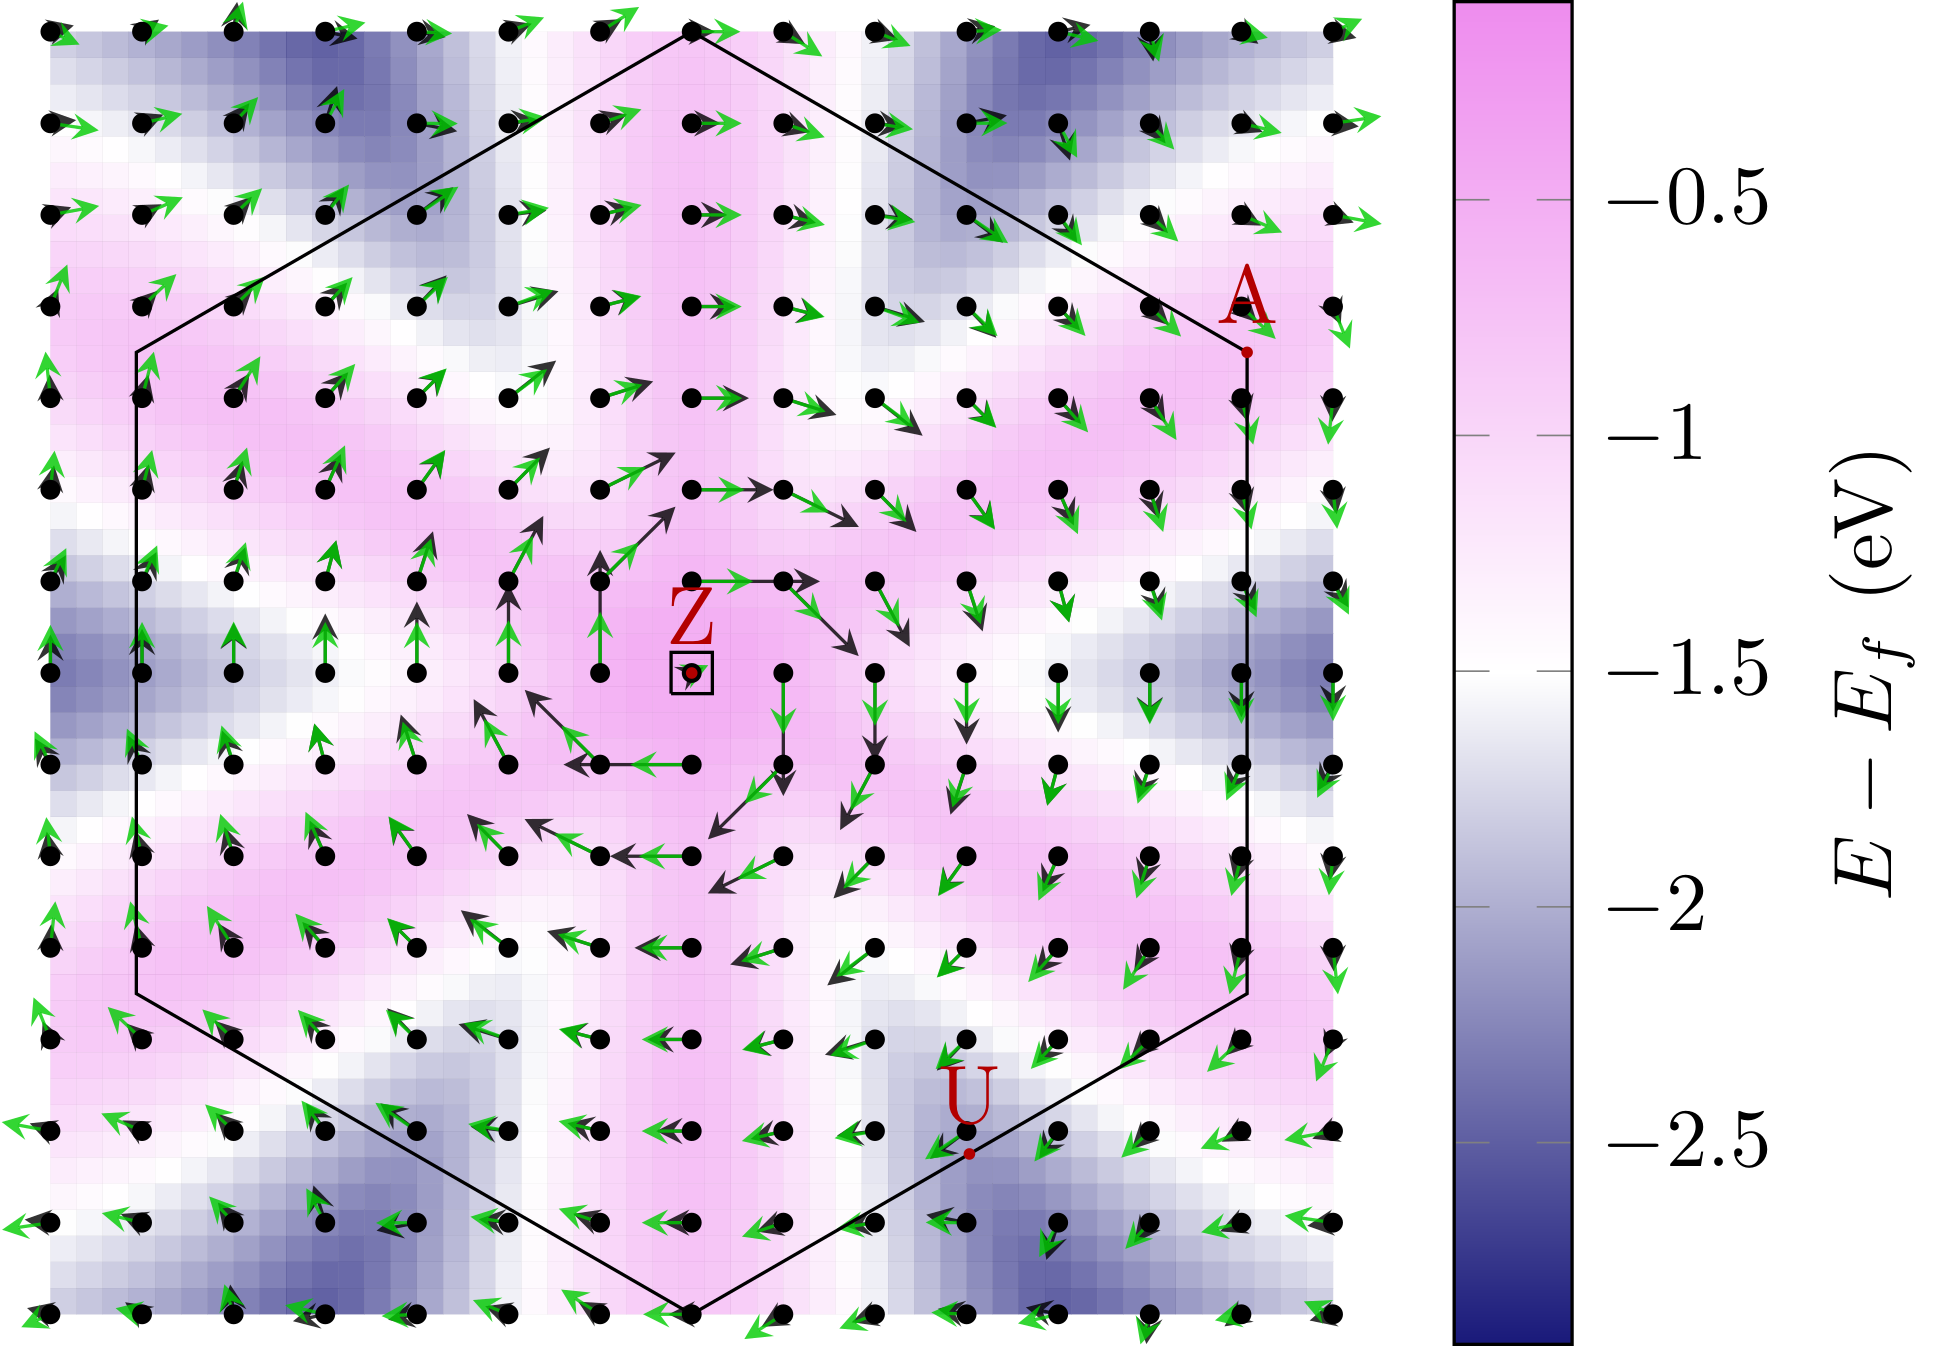
\includegraphics[width=0.32\linewidth]{Ltexture10.png}
  }
  ~
  \subfloat[Zoom-in of (d)]{
    \centering
    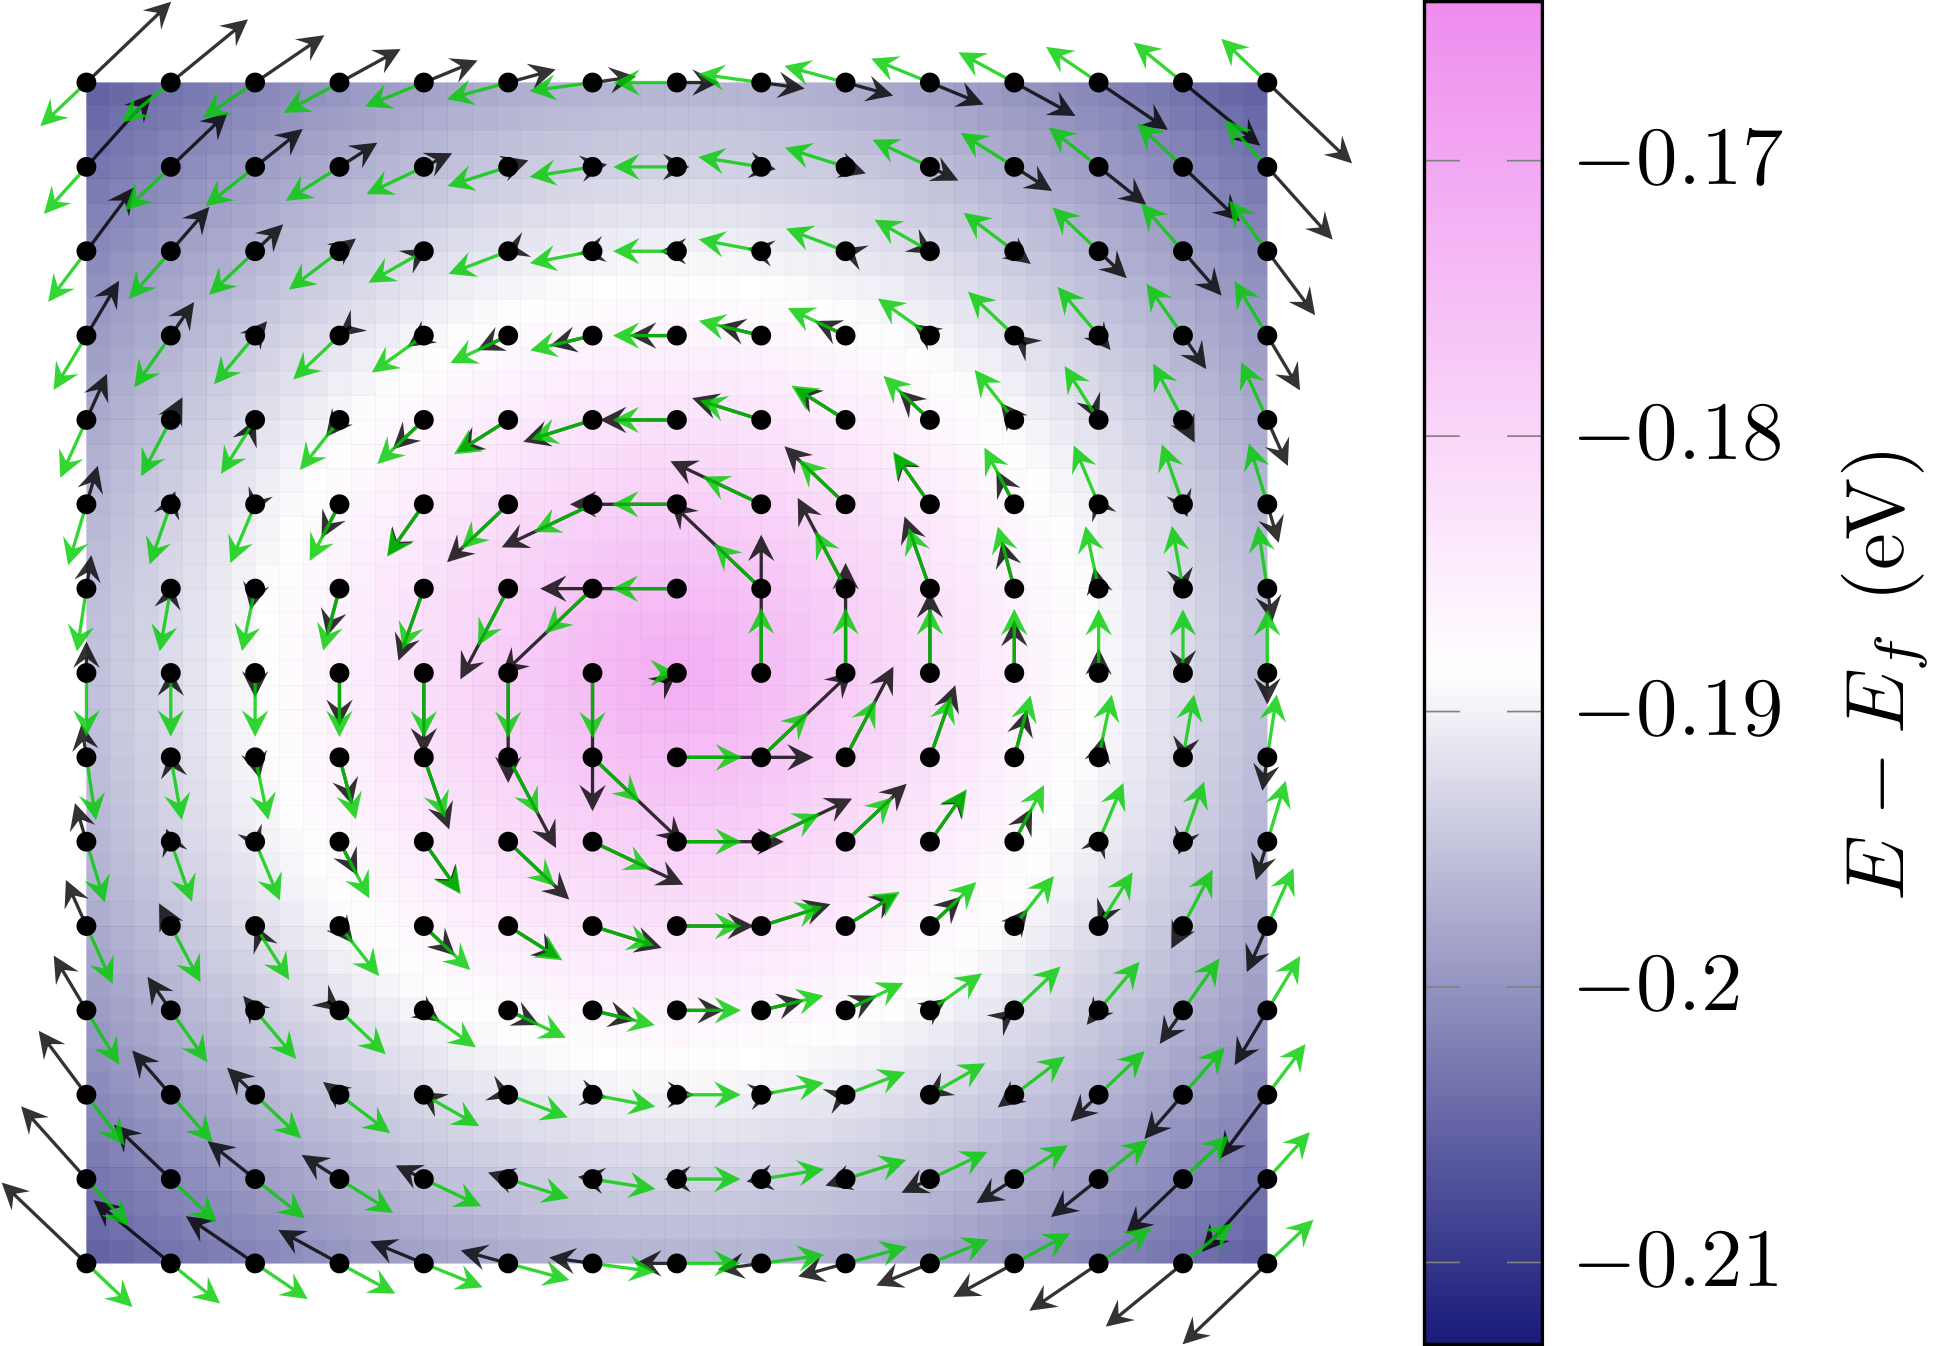
\includegraphics[width=0.34\linewidth]{Ltexture9small.png}
  }
  \caption{OAM and SAM textures around the $Z$ point in the first and third valence bands of GeTe. The black and green arrows show the OAM and SAM textures, respectively. The length of the arrows was chosen separately for clarity in each figure and should thus not be compared. The color maps signify the energy of the bands, relative to the Fermi level. The small box around the $Z$ point indicates the area, magnified in panels (c) and (f). In the zoomed figures (c) and (f) one can observe the change or relative orientation between the SAM and OAM when moving away from the $Z$ point, signifying a change of character between $j=1/2$ and $j=3/2$.}\label{fig:textures}
\end{figure*}

\section{Methods}
To back up this qualitative analysis, we performed quantitative ab initio calculations to study how the discussed effects manifest themselves in GeTe. Since we are interested in understanding the mechanism on a microscopic level, we use a tight-binding formalism based on Wannier functions \cite{Marzari2012MaximallyApplications}. The gauge freedom during the Wannierization can then be exploited to provide a set of basis functions which are localized and resemble closely the atomic orbitals (spherical harmonics). To this end we first performed a nonrelativistic DFT calculation using the Quantum-Espresso package \cite{Giannozzi2009}. We used 10x10x10 and 12x12x12 Monkhorst-Pack grids for sampling the reciprocal space in the self-consistent density and non-self-consistent calculations respectively, as well as an energy convergence threshold of $10^{-8}$~Ry in both calculations. We used ONCVPSP pseudopotentials. The energy and density cutoffs were set to 56~Ry and 500~Ry respectively.

We then employed the Wannier90 software \cite{Mostofi2014AnFunctions} to perform the Wannier interpolation of the bands close to the Fermi level, using projections onto s and p orbitals of both the Ge and Te ions. Only the projective step in the Wannierization was used to obtain Wannier functions that have the symmetry of the initial projections and therefore resemble the atomic orbitals as closely as possible. This nonetheless resulted in adequately localized Wannier functions with a total spread of 21.12 $\angstrom ^2$. The Wannier functions can then be exploited to compute how the observables of interest evolve as we progress through the Brillouin zone (BZ). There is, however, one last hurdle to overcome. We are interested in relativistic effects, therefore SOC has to be accounted for. Since at present Wannier90 can not output the Wannier functions from fully-relativistic DFT calculations, we applied the atomic SOC by adding $\lambda_{so} \bm{l} \cdot \bm{\sigma}$ term to the Wannier tight-binding Hamiltonian obtained from a collinear calculation. The matrix elements of $l$ operator were computed from the Wannier functions from the collinear calculation. $\lambda_{so}$ parameters were fitted to reproduce the band structure from a relativistic DFT calculation, resulting in $\lambda_{so}^{Te}=0.33, \lambda_{so}^{Ge}=-0.07$~eV. We only include SOC terms between Wannier functions that are centered at the same atom. This is referred to as the atomic centered approximation.

% We performed ab initio calculations to study how the discussed effects manifest themselves in GeTe. To arrive at the desired basis of Wannier functions and tight-binding Hamiltonian, we first performed a collinear DFT calculation using the Quantum-Espresso package \cite{Giannozzi2009}, followed by WANNIER90 \cite{Mostofi2014AnFunctions}. For the DFT calculation we used a 10x10x10 Monkhorst-Pack k-grid, as well as an energy convergence threshold of $10^{-8}$~Ry. In the Wannierization step the gauge freedom of Wannier functions was exploited to arrive at a set of basis functions which are localized \cite{Marzari2012MaximallyApplications}, and resemble closely the atomic orbitals (spherical harmonics). Afterwards we added atomic SOC in the form $\lambda_{so} \bm{l} \cdot \bm{\sigma}$ using the muffin-tin approximation, with $\lambda_{so}$ for both atoms used as fitting parameters. Using this basis and Hamiltonian, we can the calculate the observables of interest, namely the OAM around Te and the dipole of the Bloch functions. 
\section{Results and Discussion}
Focusing on the topmost valence band, displayed in the left panel of Fig.~\ref{fig:oamvseigvalv}, there are several features that warrant a discussion. The first is that we clearly see the linear variation of the OAM even without SOC, with forms given by Eq.~(\ref{eq:OAM}). Secondly, since only $k_y$ varies along the $A \to Z$ path, it it evident that the OAM along the $y$ axis ($l_y$) vanishes along the entire path. It is only when $k_x$ varies, as the wavevector progresses along the $Z \to U$ path, that we observe a nonvanishing $l_y$. Along this path, the sign of $k_x$ is negative whereas the sign of $k_y$ is positive just as along the $Z-A$ path. This results in a consistent orientation of $l_y$ and $l_x$, given by Eq.~(\ref{eq:OAM}). The third observation is that including atomic SOC is manifestated in the "unquenching" of the OAM. In Fig.~\ref{fig:oamvseigvalv}, as soon as there is an infinitesimal variation of the the wave vector from the time-reversal invariant $Z$-point (where $\bm{l}=0$ due to the symmetry), the unquenching of OAM leads to a nonzero shift in the OAM, with the sign depending on the subband.

Lastly, to correlate the changes in the OAM and the dipole of the Bloch function, we computed the $z$ coordinate of the center of mass $\bar{z}=\int_{\textrm{supercell}}z |\psi(k)|^2$, which is proportional to the dipole moment computed around the same reference point. Figure ~\ref{fig:oamvseigvalv} shows the  correlation of the dipole and OAM of the bands, consistent with Eq.~(\ref{eq:dipfinal}), while Fig.~\ref{Fig:diffdens} displays the asymmetric variation of the charge density of the first valence band along the $Z\to A$ path. More specifically, there is a clear development of a nonzero dipole moment around Ge, which couples to the local $E_z$.
These considerations also hold true for the third valence band, as seen from the right panel of Fig.~\ref{fig:oamvseigvalv}.

In addition to the magnitude of $\alpha_R$,  other important features are dependent on the orbital character of the bands, unlike in the case of the relativistic Rashba effect, as was discussed above. We see that for states with predominant $j=\frac{3}{2}$ or $j=\frac{1}{2}$ character, the SAM is oriented along or opposite to the OAM, respectively. Comparing the orientations of the SAM and OAM, shown in Fig.~\ref{fig:textures}, we conclude that close to the $Z$-point, the topmost valence band has mostly $j=\frac{3}{2}$ character, whereas the third mostly $j=\frac{1}{2}$.
Interestingly, the states in the upper third valence band and lower first valence band switch characters when moving further away from the $Z$ point, as seen in the panels (c) and (f) of Fig.~\ref{fig:textures}. This draws attention to the fact that inclusion of Eq.~(\ref{HOR}) breaks threefold symmetry and results in $j$ not being a good quantum number anymore. This causes a highly nontrivial SAM and OAM texture to be present in these two subbands, with both SAM and OAM varying considerably throughout the BZ.
When comparing the spin splitting of the two valence bands, their relative signs are opposite, an effect which cannot be explained by the relativistic Rashba effect [Eq.~(\ref{eq:relrashba})], that leads to the same splittings, regardless of the character of the band. Only terms such as Eq.~(\ref{eq:dipfinal}) can explain this behavior.

%Looking back to Eq.~(\ref{eq:hami}), we can identify three main mechanisms that can result in a large linear spin splitting in the band dispersion.
  %The first is large OAM unquenching effect, resulting in a significant $\bm{l}(Z)$ which couples to $\bm{\sigma}(Z)$, causing a linear variation of the dipole energy through the first term of Eq.~(\ref{eq:dipfinal}). The second is a linear variation of OAM a constant SAM, and the third -- vice versa. 
%In the topmost valence band the linear variations of the dipole and SAM are very small. This suggests that the origin of the giant Rashba-like splitting is the large linear variation of the OAM, caused by the coupling to the electric polarization through the dipole, together with the large atomic SOC which then couples to the nonzero SAM through $\lambda_{so} \bm{l} \cdot \bm{\sigma}$. In the third valence band, however, the variation of the OAM is less than that of the SAM, and the contribution due to the charge asymmetry plays a bigger role, making it hard to assign the splitting to a single contribution. 

\section{Conclusions}

We have explored the microscopic origin of the giant Rashba-like spin splitting in the band structure of bulk ferroelectric GeTe with high atomic SOC. We derived the form of the band dispersion in the Wannier representation, that relates the large spin splitting to the intricate interplay between OAM, atomic SOC, the crystal field and the electric polarization. It turns out that the crucial component, which is not present in the relativistic Rashba effect, is the emergence of a nonzero electric dipole of the Bloch functions due to their OAM. The quantitative analysis based on Wannier functions and atomic-centered approximation confirms this mechanism in GeTe. We find a very good agreement between the proposed band dispersion, Eq.~(\ref{eq:hami}), and the dispersions of the first and third valence bands, where the effect manifests itself most clearly.

Ultimately, the results suggest that (1) large ferroelectric polarization, (2) high atomic SOC, and (3) highly symmetric environment producing little OAM quenching could be the design rules for new materials with strong Rashba-like spin splitting. These materials could enable spintronic devices with the much needed electric control of spin polarization.

% \bibliography{000Mendeley}%

%merlin.mbs apsrev4-1.bst 2010-07-25 4.21a (PWD, AO, DPC) hacked
%Control: key (0)
%Control: author (8) initials jnrlst
%Control: editor formatted (1) identically to author
%Control: production of article title (-1) disabled
%Control: page (0) single
%Control: year (1) truncated
%Control: production of eprint (0) enabled
\begin{thebibliography}{20}%
\makeatletter
\providecommand \@ifxundefined [1]{%
 \@ifx{#1\undefined}
}%
\providecommand \@ifnum [1]{%
 \ifnum #1\expandafter \@firstoftwo
 \else \expandafter \@secondoftwo
 \fi
}%
\providecommand \@ifx [1]{%
 \ifx #1\expandafter \@firstoftwo
 \else \expandafter \@secondoftwo
 \fi
}%
\providecommand \natexlab [1]{#1}%
\providecommand \enquote  [1]{``#1''}%
\providecommand \bibnamefont  [1]{#1}%
\providecommand \bibfnamefont [1]{#1}%
\providecommand \citenamefont [1]{#1}%
\providecommand \href@noop [0]{\@secondoftwo}%
\providecommand \href [0]{\begingroup \@sanitize@url \@href}%
\providecommand \@href[1]{\@@startlink{#1}\@@href}%
\providecommand \@@href[1]{\endgroup#1\@@endlink}%
\providecommand \@sanitize@url [0]{\catcode `\\12\catcode `\$12\catcode
  `\&12\catcode `\#12\catcode `\^12\catcode `\_12\catcode `\%12\relax}%
\providecommand \@@startlink[1]{}%
\providecommand \@@endlink[0]{}%
\providecommand \url  [0]{\begingroup\@sanitize@url \@url }%
\providecommand \@url [1]{\endgroup\@href {#1}{\urlprefix }}%
\providecommand \urlprefix  [0]{URL }%
\providecommand \Eprint [0]{\href }%
\providecommand \doibase [0]{http://dx.doi.org/}%
\providecommand \selectlanguage [0]{\@gobble}%
\providecommand \bibinfo  [0]{\@secondoftwo}%
\providecommand \bibfield  [0]{\@secondoftwo}%
\providecommand \translation [1]{[#1]}%
\providecommand \BibitemOpen [0]{}%
\providecommand \bibitemStop [0]{}%
\providecommand \bibitemNoStop [0]{.\EOS\space}%
\providecommand \EOS [0]{\spacefactor3000\relax}%
\providecommand \BibitemShut  [1]{\csname bibitem#1\endcsname}%
\let\auto@bib@innerbib\@empty
%</preamble>
\bibitem [{\citenamefont {Datta}\ and\ \citenamefont {Das}(1990)}]{Datta1990}%
  \BibitemOpen
  \bibfield  {author} {\bibinfo {author} {\bibfnamefont {S.}~\bibnamefont
  {Datta}}\ and\ \bibinfo {author} {\bibfnamefont {B.}~\bibnamefont {Das}},\
  }\href {\doibase 10.1063/1.102730} {\bibfield  {journal} {\bibinfo  {journal}
  {Applied Physics Letters}\ }\textbf {\bibinfo {volume} {56}},\ \bibinfo
  {pages} {665} (\bibinfo {year} {1990})}\BibitemShut {NoStop}%
\bibitem [{\citenamefont {Kent}\ and\ \citenamefont
  {Worledge}(2015)}]{Kent2015}%
  \BibitemOpen
  \bibfield  {author} {\bibinfo {author} {\bibfnamefont {A.~D.}\ \bibnamefont
  {Kent}}\ and\ \bibinfo {author} {\bibfnamefont {D.~C.}\ \bibnamefont
  {Worledge}},\ }\href {\doibase 10.1038/nnano.2015.24} {\bibfield  {journal}
  {\bibinfo  {journal} {Nature Nanotechnology}\ }\textbf {\bibinfo {volume}
  {10}},\ \bibinfo {pages} {187} (\bibinfo {year} {2015})}\BibitemShut
  {NoStop}%
\bibitem [{\citenamefont {Jungwirth}\ \emph {et~al.}(2016)\citenamefont
  {Jungwirth}, \citenamefont {Marti}, \citenamefont {Wadley},\ and\
  \citenamefont {Wunderlich}}]{Jungwirth2016}%
  \BibitemOpen
  \bibfield  {author} {\bibinfo {author} {\bibfnamefont {T.}~\bibnamefont
  {Jungwirth}}, \bibinfo {author} {\bibfnamefont {X.}~\bibnamefont {Marti}},
  \bibinfo {author} {\bibfnamefont {P.}~\bibnamefont {Wadley}}, \ and\ \bibinfo
  {author} {\bibfnamefont {J.}~\bibnamefont {Wunderlich}},\ }\href {\doibase
  10.1038/nnano.2016.18} {\bibfield  {journal} {\bibinfo  {journal} {Nature
  Nanotechnology}\ }\textbf {\bibinfo {volume} {11}},\ \bibinfo {pages} {231}
  (\bibinfo {year} {2016})}\BibitemShut {NoStop}%
\bibitem [{\citenamefont {Di~Sante}\ \emph {et~al.}(2013)\citenamefont
  {Di~Sante}, \citenamefont {Barone}, \citenamefont {Bertacco},\ and\
  \citenamefont {Picozzi}}]{DiSante2013}%
  \BibitemOpen
  \bibfield  {author} {\bibinfo {author} {\bibfnamefont {D.}~\bibnamefont
  {Di~Sante}}, \bibinfo {author} {\bibfnamefont {P.}~\bibnamefont {Barone}},
  \bibinfo {author} {\bibfnamefont {R.}~\bibnamefont {Bertacco}}, \ and\
  \bibinfo {author} {\bibfnamefont {S.}~\bibnamefont {Picozzi}},\ }\href
  {\doibase 10.1002/adma.201203199} {\bibfield  {journal} {\bibinfo  {journal}
  {Advanced Materials}\ }\textbf {\bibinfo {volume} {25}},\ \bibinfo {pages}
  {509} (\bibinfo {year} {2013})}\BibitemShut {NoStop}%
\bibitem [{\citenamefont {Ishizaka}(2011)}]{Ishizaka2011}%
  \BibitemOpen
  \bibfield  {author} {\bibinfo {author} {\bibfnamefont {K.}~\bibnamefont
  {Ishizaka}},\ }\href {\doibase 10.1038/nmat3051} {\bibfield  {journal}
  {\bibinfo  {journal} {Nature materials}\ }\textbf {\bibinfo {volume} {10}},\
  \bibinfo {pages} {521} (\bibinfo {year} {2011})}\BibitemShut {NoStop}%
\bibitem [{\citenamefont {Kim}\ \emph {et~al.}(2014)\citenamefont {Kim},
  \citenamefont {Im}, \citenamefont {Freeman}, \citenamefont {Ihm},\ and\
  \citenamefont {Jin}}]{Kim2014}%
  \BibitemOpen
  \bibfield  {author} {\bibinfo {author} {\bibfnamefont {M.}~\bibnamefont
  {Kim}}, \bibinfo {author} {\bibfnamefont {J.}~\bibnamefont {Im}}, \bibinfo
  {author} {\bibfnamefont {A.~J.}\ \bibnamefont {Freeman}}, \bibinfo {author}
  {\bibfnamefont {J.}~\bibnamefont {Ihm}}, \ and\ \bibinfo {author}
  {\bibfnamefont {H.}~\bibnamefont {Jin}},\ }\href {\doibase
  10.1073/pnas.1405780111} {\bibfield  {journal} {\bibinfo  {journal}
  {Proceedings of the National Academy of Sciences of the United States of
  America}\ }\textbf {\bibinfo {volume} {111}},\ \bibinfo {pages} {6900}
  (\bibinfo {year} {2014})}\BibitemShut {NoStop}%
\bibitem [{\citenamefont {Liebmann}\ \emph {et~al.}(2016)\citenamefont
  {Liebmann}, \citenamefont {Rinaldi}, \citenamefont {Di~Sante}, \citenamefont
  {Kellner}, \citenamefont {Pauly}, \citenamefont {Wang}, \citenamefont
  {Boschker}, \citenamefont {Giussani}, \citenamefont {Bertoli}, \citenamefont
  {Cantoni}, \citenamefont {Baldrati}, \citenamefont {Asa}, \citenamefont
  {Vobornik}, \citenamefont {Panaccione}, \citenamefont {Marchenko},
  \citenamefont {Sanchez-Barriga}, \citenamefont {Rader}, \citenamefont
  {Calarco}, \citenamefont {Picozzi}, \citenamefont {Bertacco},\ and\
  \citenamefont {Morgenstern}}]{Liebmann2016}%
  \BibitemOpen
  \bibfield  {author} {\bibinfo {author} {\bibfnamefont {M.}~\bibnamefont
  {Liebmann}}, {\bibfnamefont {C.}~\bibnamefont{Rinaldi}}, {\bibfnamefont {D.}~\bibnamefont{Di Sante}},
  {\bibfnamefont {J.}~\bibnamefont{Kellner}}, {\bibfnamefont {C.}~\bibnamefont{Pauly}}, {\bibfnamefont {R. N.}~\bibnamefont{Wang}},
  {\bibfnamefont {J. E.}~\bibnamefont{Boschker}}, {\bibfnamefont {A.}~\bibnamefont{Giussani}}, {\bibfnamefont {S.}~\bibnamefont{Bertoli}},
  {\bibfnamefont {M.}~\bibnamefont{Cantoni}}, {\bibfnamefont {L.}~\bibnamefont{Baldrati}},
  {\bibfnamefont {M.}~\bibnamefont{Asa}}, {\bibfnamefont {I.}~\bibnamefont{Vobornik}}, {\bibfnamefont {G.}~\bibnamefont{Panaccione}},
  {\bibfnamefont {D.}~\bibnamefont{Marchenko}}, {\bibfnamefont {J.}~\bibnamefont{S\'anchez-Barriga}}, 
  {\bibfnamefont {O.}~\bibnamefont{Rader}}, {\bibfnamefont {R.}~\bibnamefont{Calarco}}, {\bibfnamefont {S.}~\bibnamefont{Picozzi}},
  {\bibfnamefont {R.}~\bibnamefont{Bertacco}}, {\bibfnamefont {M.}~\bibnamefont{Morgenstern}}  
  {\it et~al.},\ }\href {\doibase 10.1002/adma.201503459}
  {\bibfield  {journal} {\bibinfo  {journal} {Advanced Materials}\ }\textbf
  {\bibinfo {volume} {28}},\ \bibinfo {pages} {560} (\bibinfo {year}
  {2016})}\BibitemShut {NoStop}%
\bibitem [{\citenamefont {Krempask{\'{y}}}, {\it et~al.}(2016)\citenamefont
  {Krempask{\'{y}}}, \citenamefont {Volfov{\'{a}}}, \citenamefont {Muff},
  \citenamefont {Pilet}, \citenamefont {Landolt}, \citenamefont
  {Radovi{\'{c}}}, \citenamefont {Shi}, \citenamefont {Kriegner}, \citenamefont
  {Hol{\'{y}}}, \citenamefont {Braun}, \citenamefont {Ebert}, \citenamefont
  {Bisti}, \citenamefont {Rogalev}, \citenamefont {Strocov}, \citenamefont
  {Springholz}, \citenamefont {Min{\'{a}}r},\ and\ \citenamefont
  {Dil}}]{Krempasky2015SurfaceSemiconductor}%
  \BibitemOpen
  \bibfield  {author} {\bibinfo {author} {\bibfnamefont {J.}~\bibnamefont
  {Krempask{\'{y}}}}, {\bibfnamefont {H.}~\bibnamefont
  {Volfov\'a}}, {\bibfnamefont {S.}~\bibnamefont
  {Muff}}, {\bibfnamefont {N.}~\bibnamefont
  {Pilet}}, {\bibfnamefont {G.}~\bibnamefont
  {Landolt}}, {\bibfnamefont {M.}~\bibnamefont
  {Radovi\'c}}, {\bibfnamefont {M.}~\bibnamefont
  {Shi}}, {\bibfnamefont {D.}~\bibnamefont
  {Kriegner}}, {\bibfnamefont {V.}~\bibnamefont
  {Hol\'y}}, {\bibfnamefont {J.}~\bibnamefont
  {Braun}}, {\bibfnamefont {H.}~\bibnamefont
  {Ebert}}, {\bibfnamefont {F.}~\bibnamefont
  {Bisti}}, {\bibfnamefont {V. A.}~\bibnamefont
  {Rogalev}}, {\bibfnamefont {V. N.}~\bibnamefont
  {Strocov}}, {\bibfnamefont {G.}~\bibnamefont
  {Springholz}}, {\bibfnamefont {J.}~\bibnamefont
  {Min\'ar}}, {\bibfnamefont {J. H.}~\bibnamefont
  {Dil}}, }\href {\doibase 10.1103/PhysRevB.94.205111}
  {\bibfield  {journal} {\bibinfo  {journal} {Phys. Rev. B}\ }\textbf
  {\bibinfo {volume} {94}},\ \bibinfo {pages} {205111} (\bibinfo {year} 
  {2016})}\BibitemShut {NoStop}%
  
\bibitem [{\citenamefont {Rashba}\ and\ \citenamefont
  {Sheka}(1959)}]{Rashba1959SymmetryAr}%
  \BibitemOpen
  \bibfield  {author} {\bibinfo {author} {\bibfnamefont {E.}~\bibnamefont
  {Rashba}}\ and\ \bibinfo {author} {\bibfnamefont {V.}~\bibnamefont {Sheka}},\
  }\href {http://nrs.harvard.edu/urn-3:HUL.InstRepos:29426010} {\bibfield  {journal} {\bibinfo  {journal} {New. J. Phys.} \textbf{\bibinfo{volume}{17}},\ \bibinfo {pages} {050202}} (\bibinfo {year}
  {2015})}\BibitemShut {NoStop}%
\bibitem [{\citenamefont {Lifshitz}\ \emph {et~al.}(1982)\citenamefont
  {Lifshitz}, \citenamefont {Berestetskii},\ and\ \citenamefont
  {Pitaevskii}}]{Lifshitz1982CourseTheory}%
  \BibitemOpen
  \bibfield  {author} {\bibinfo {author} {\bibfnamefont {E.~M.}\ \bibnamefont
  {Lifshitz}}, \bibinfo {author} {\bibfnamefont {V.~B.}\ \bibnamefont
  {Berestetskii}}, \ and\ \bibinfo {author} {\bibfnamefont {L.~P.}\
  \bibnamefont {Pitaevskii}},\ }\href {http://ci.nii.ac.jp/ncid/BA20776995}
  {\bibinfo {title} \it Course of Theoretical Physics - Volume 4:
  Relativistic Quantum Theory},\ \bibinfo {edition} {2nd}\ ed.\ (\bibinfo
  {publisher} {Elsevier, Oxford},\ \bibinfo {year} {1982})\BibitemShut {NoStop}%
\bibitem [{\citenamefont {Rabe}\ and\ \citenamefont
  {Joannopoulos}(1987)}]{Rabe1987}%
  \BibitemOpen
  \bibfield  {author} {\bibinfo {author} {\bibfnamefont {K.~M.}\ \bibnamefont
  {Rabe}}\ and\ \bibinfo {author} {\bibfnamefont {J.~D.}\ \bibnamefont
  {Joannopoulos}},\ }\href {\doibase 10.1103/PhysRevB.36.6631} {\bibfield
  {journal} {\bibinfo  {journal} {Phys. Rev. B}\ }\textbf {\bibinfo
  {volume} {36}},\ \bibinfo {pages} {6631} (\bibinfo {year}
  {1987})}\BibitemShut {NoStop}%
\bibitem [{\citenamefont {Garrity}\ \emph {et~al.}(2014)\citenamefont
  {Garrity}, \citenamefont {Rabe},\ and\ \citenamefont
  {Vanderbilt}}]{Garrity2013Hyperferroelectrics:Polarization}%
  \BibitemOpen
  \bibfield  {author} {\bibinfo {author} {\bibfnamefont {K.~F.}\ \bibnamefont
  {Garrity}}, \bibinfo {author} {\bibfnamefont {K.~M.}\ \bibnamefont {Rabe}}, \
  and\ \bibinfo {author} {\bibfnamefont {D.}~\bibnamefont {Vanderbilt}},\
  }\href {\doibase 10.1103/PhysRevLett.112.127601} {\bibfield  {journal}
  {\bibinfo  {journal} {Phys. Rev. Lett.}\ }\textbf {\bibinfo {volume}
  {112}},\ \bibinfo {pages} {127601} (\bibinfo {year} {2014})}\BibitemShut {NoStop}%
\bibitem [{\citenamefont {Meyer}\ and\ \citenamefont
  {Vanderbilt}(2001)}]{Meyer2008AbFields}%
  \BibitemOpen
  \bibfield  {author} {\bibinfo {author} {\bibfnamefont {B.}~\bibnamefont
  {Meyer}}\ and\ \bibinfo {author} {\bibfnamefont {D.}~\bibnamefont
  {Vanderbilt}},\ } \href {\doibase 10.1103/PhysRevB.63.205426} {\bibfield      {journal}
  {\bibinfo  {journal} {Phys. Rev. B}\ }\textbf {\bibinfo {volume}{63}},\ \bibinfo    {pages} {205426} (\bibinfo {year} {2001})}\BibitemShut {NoStop}%
\bibitem [{\citenamefont {Park}\ \emph {et~al.}(2011)\citenamefont {Park},
  \citenamefont {Kim}, \citenamefont {Yu}, \citenamefont {Han},\ and\
  \citenamefont {Kim}}]{Park2011}%
  \BibitemOpen
  \bibfield  {author} {\bibinfo {author} {\bibfnamefont {S.~R.}\ \bibnamefont
  {Park}}, \bibinfo {author} {\bibfnamefont {C.~H.}\ \bibnamefont {Kim}},
  \bibinfo {author} {\bibfnamefont {J.}~\bibnamefont {Yu}}, \bibinfo {author}
  {\bibfnamefont {J.~H.}\ \bibnamefont {Han}}, \ and\ \bibinfo {author}
  {\bibfnamefont {C.}~\bibnamefont {Kim}},\ }\href {\doibase
  10.1103/PhysRevLett.107.156803} {\bibfield  {journal} {\bibinfo  {journal}
  {Phys. Rev. Lett.}\ }\textbf {\bibinfo {volume} {107}},\ \bibinfo
  {pages} {156803} (\bibinfo {year} {2011})}\BibitemShut {NoStop}%
\bibitem [{\citenamefont {Park}\ \emph {et~al.}(2012)\citenamefont {Park},
  \citenamefont {Kim}, \citenamefont {Rhim},\ and\ \citenamefont
  {Han}}]{Park2012}%
  \BibitemOpen
  \bibfield  {author} {\bibinfo {author} {\bibfnamefont {J.~H.}\ \bibnamefont
  {Park}}, \bibinfo {author} {\bibfnamefont {C.~H.}\ \bibnamefont {Kim}},
  \bibinfo {author} {\bibfnamefont {J.~W.}\ \bibnamefont {Rhim}}, \ and\
  \bibinfo {author} {\bibfnamefont {J.~H.}\ \bibnamefont {Han}},\ }\href
  {\doibase 10.1103/PhysRevB.85.195401} {\bibfield  {journal} {\bibinfo
  {journal} {Phys. Rev. B}\
  }\textbf {\bibinfo {volume} {85}},\ \bibinfo {pages} {195401} (\bibinfo {year}
  {2012})}\BibitemShut {NoStop}%
\bibitem [{\citenamefont {Park}\ and\ \citenamefont
  {Kim}(2015)}]{Park2015MicroscopicMomentum}%
  \BibitemOpen
  \bibfield  {author} {\bibinfo {author} {\bibfnamefont {S.~R.}\ \bibnamefont
  {Park}}\ and\ \bibinfo {author} {\bibfnamefont {C.}~\bibnamefont {Kim}},\
  }\href {\doibase 10.1016/j.elspec.2014.12.009} {\bibfield  {journal}
  {\bibinfo  {journal} {J. Electron. Spectros. Relat. Phenomena}\ }\textbf {\bibinfo {volume} {201}},\ \bibinfo {pages} {6}
  (\bibinfo {year} {2015})}\BibitemShut {NoStop}%
\bibitem [{\citenamefont {Hong}\ \emph {et~al.}(2015)\citenamefont {Hong},
  \citenamefont {Rhim}, \citenamefont {Kim}, \citenamefont {Ryong~Park},\ and\
  \citenamefont {Hoon~Shim}}]{Hong2015QuantitativeSplitting}%
  \BibitemOpen
  \bibfield  {author} {\bibinfo {author} {\bibfnamefont {J.}~\bibnamefont
  {Hong}}, \bibinfo {author} {\bibfnamefont {J.-W.}\ \bibnamefont {Rhim}},
  \bibinfo {author} {\bibfnamefont {C.}~\bibnamefont {Kim}}, \bibinfo {author}
  {\bibfnamefont {S.}~\bibnamefont {Ryong~Park}}, \ and\ \bibinfo {author}
  {\bibfnamefont {J.}~\bibnamefont {Hoon~Shim}},\ }\href {\doibase
  10.1038/srep13488} {\bibfield  {journal} {\bibinfo  {journal} {Sci.
  Rep.}\ }\textbf {\bibinfo {volume} {5}},\ \bibinfo {pages} {13488}
  (\bibinfo {year} {2015})}\BibitemShut {NoStop}%
\bibitem [{\citenamefont {Marzari}\ \emph {et~al.}(2012)\citenamefont
  {Marzari}, \citenamefont {Mostofi}, \citenamefont {Yates}, \citenamefont
  {Souza},\ and\ \citenamefont
  {Vanderbilt}}]{Marzari2012MaximallyApplications}%
  \BibitemOpen
  \bibfield  {author} {\bibinfo {author} {\bibfnamefont {N.}~\bibnamefont
  {Marzari}}, \bibinfo {author} {\bibfnamefont {A.~A.}\ \bibnamefont
  {Mostofi}}, \bibinfo {author} {\bibfnamefont {J.~R.}\ \bibnamefont {Yates}},
  \bibinfo {author} {\bibfnamefont {I.}~\bibnamefont {Souza}}, \ and\ \bibinfo
  {author} {\bibfnamefont {D.}~\bibnamefont {Vanderbilt}},\ }\href {\doibase
  10.1103/RevModPhys.84.1419} {\bibfield  {journal} {\bibinfo  {journal}
  {Rev. Mod. Phys.}\ }\textbf {\bibinfo {volume} {84}},\ \bibinfo
  {pages} {1419} (\bibinfo {year} {2012})}\BibitemShut {NoStop}%
\bibitem [{\citenamefont {Petersen}\ and\ \citenamefont
  {Hedeg{\aa}rd}(2000)}]{Petersen2000SimpleStates}%
  \BibitemOpen
  \bibfield  {author} {\bibinfo {author} {\bibfnamefont {L.}~\bibnamefont
  {Petersen}}\ and\ \bibinfo {author} {\bibfnamefont {P.}~\bibnamefont
  {Hedeg{\aa}rd}},\ }\href {\doibase 10.1016/S0039-6028(00)00441-6} {\bibfield
  {journal} {\bibinfo  {journal} {Surf. Sci.}\ }\textbf {\bibinfo {volume}
  {459}},\ \bibinfo {pages} {49} (\bibinfo {year} {2000})}\BibitemShut
  {NoStop}%
\bibitem [{\citenamefont {Go}\ \emph {et~al.}(2016)\citenamefont {Go},
  \citenamefont {Hanke}, \citenamefont {Buhl}, \citenamefont {Freimuth},
  \citenamefont {Bihlmayer}, \citenamefont {Lee}, \citenamefont {Mokrousov},\
  and\ \citenamefont {Bl{\"{u}}gel}}]{Go2016SurfacePhysics}%
  \BibitemOpen
  \bibfield  {author} {\bibinfo {author} {\bibfnamefont {D.}~\bibnamefont
  {Go}}, \bibinfo {author} {\bibfnamefont {J.-P.}\ \bibnamefont {Hanke}},
  \bibinfo {author} {\bibfnamefont {P.~M.}\ \bibnamefont {Buhl}}, \bibinfo
  {author} {\bibfnamefont {F.}~\bibnamefont {Freimuth}}, \bibinfo {author}
  {\bibfnamefont {G.}~\bibnamefont {Bihlmayer}}, \bibinfo {author}
  {\bibfnamefont {H.-W.}\ \bibnamefont {Lee}}, \bibinfo {author} {\bibfnamefont
  {Y.}~\bibnamefont {Mokrousov}}, \ and\ \bibinfo {author} {\bibfnamefont
  {S.}~\bibnamefont {Bl{\"{u}}gel}},\ }\href {\doibase 10.1038/srep46742} 		
  {\bibfield
  {journal} {\bibinfo  {journal} {Sci. Rep.}\ }\textbf {\bibinfo {volume}
  {7}},\ \bibinfo {pages} {46742} (\bibinfo {year} {2017})}\BibitemShut {NoStop}%
\bibitem [{\citenamefont {Giannozzi}\ \emph {et~al.}(2009)\citenamefont
  {Giannozzi}, \citenamefont {Baroni}, \citenamefont {Bonini}, \citenamefont
  {Calandra}, \citenamefont {Car}, \citenamefont {Cavazzoni}, \citenamefont
  {Ceresoli}, \citenamefont {Chiarotti}, \citenamefont {Cococcioni},
  \citenamefont {Dabo}, \citenamefont {Dal~Corso}, \citenamefont
  {de~Gironcoli}, \citenamefont {Fabris}, \citenamefont {Fratesi},
  \citenamefont {Gebauer}, \citenamefont {Gerstmann}, \citenamefont
  {Gougoussis}, \citenamefont {Kokalj}, \citenamefont {Lazzeri}, \citenamefont
  {Martin-Samos}, \citenamefont {Marzari}, \citenamefont {Mauri}, \citenamefont
  {Mazzarello}, \citenamefont {Paolini}, \citenamefont {Pasquarello},
  \citenamefont {Paulatto}, \citenamefont {Sbraccia}, \citenamefont {Scandolo},
  \citenamefont {Sclauzero}, \citenamefont {Seitsonen}, \citenamefont
  {Smogunov}, \citenamefont {Umari},\ and\ \citenamefont
  {Wentzcovitch}}]{Giannozzi2009}%
  \BibitemOpen
  \bibfield  {author} {\bibinfo {author} {\bibfnamefont {P.}~\bibnamefont
  {Giannozzi}}, {\it et~al.}}\href {\doibase 10.1088/0953-8984/21/39/395502} {\bibfield  {journal}
  {\bibinfo  {journal} {J. Phys.: Cond. Mat.}\ }\textbf {\bibinfo {volume} {21}},\ \bibinfo {pages}
  {395502} (\bibinfo {year} {2009})}\BibitemShut {NoStop}%
\bibitem [{\citenamefont {Mostofi}\ \emph {et~al.}(2014)\citenamefont
  {Mostofi}, \citenamefont {Yates}, \citenamefont {Pizzi}, \citenamefont {Lee},
  \citenamefont {Souza}, \citenamefont {Vanderbilt},\ and\ \citenamefont
  {Marzari}}]{Mostofi2014AnFunctions}%
  \BibitemOpen
  \bibfield  {author} {\bibinfo {author} {\bibfnamefont {A.~A.}\ \bibnamefont
  {Mostofi}}, \bibinfo {author} {\bibfnamefont {J.~R.}\ \bibnamefont {Yates}},
  \bibinfo {author} {\bibfnamefont {G.}~\bibnamefont {Pizzi}}, \bibinfo
  {author} {\bibfnamefont {Y.~S.}\ \bibnamefont {Lee}}, \bibinfo {author}
  {\bibfnamefont {I.}~\bibnamefont {Souza}}, \bibinfo {author} {\bibfnamefont
  {D.}~\bibnamefont {Vanderbilt}}, \ and\ \bibinfo {author} {\bibfnamefont
  {N.}~\bibnamefont {Marzari}},\ }\href {\doibase 10.1016/j.cpc.2014.05.003}
  {\bibfield  {journal} {\bibinfo  {journal} {Comp. Phys. Comm.}\
  }\textbf {\bibinfo {volume} {185}},\ \bibinfo {pages} {2309} (\bibinfo {year}
  {2014})}\BibitemShut {NoStop}%
\end{thebibliography}%

\end{document}
%























% ****** End of file apssamp.tex ******
